\chapter{Signal Extraction}\label{ch:sig}
\section{Fit Model}\label{ch:sig:fit}
The cross sections of the \Wpm and \Z bosons are determined by a simultaneous fit of \Wp, \Wm, and \Z boson channels. Modeled observable distributions of \Wp, \Wm, and \Z boson signals and associated backgrounds are fit to their respective observable distribution in data. The discriminant for the \Wp and \Wm bosons is the transverse mass (\mt) observable, and for \Z bosons is the dilepton invariant mass \mll. Equation~\ref{eq:mt} shows the definition of \mt.
\begin{equation}
\mt = \sqrt{ 2 \pt^{\ell} \met ( 1 - \cos[\Delta\phi( {\vec \ell},\met ) ] ) }
\label{eq:mt}
\end{equation}

The \mll and \mt distributions for the \Wp, \Wm, and \Z boson signal processes as well as their backgrounds are modeled as described in the following section. 
The full fit model consists of the \Wp, \Wm, and \Z boson signal models, the diboson background, the \ttbar background, the Drell-Yan background, and the $W$+jets background. The \Wp and \Wm boson channels also include a QCD background. All signal and background models include the appropriate correction, which affect the discriminant distribution and overall normalizations. Detailed descriptions of the background processes and modeling are provided in the next section, the remainder of this section describes how these are incorporated into the  fit. 
\subsubsection{Normalizations}
Signal process normalizations are independent across channels. Within a given channel, the signal process and background process from the same production mechanism (i.e. \wmunu and \wtau) have their rates fixed relative to each other. The \ttbar normalizations and diboson normalizations are fully correlated across the \Wp, \Wm, and \Z boson channels. Uncertainties in the normalizations of each of these processes is set to $10\%$. The Drell-Yan background normalization is correlated between the \Wp and \Wm boson channels, with a normalization uncertainty of $3\%$. QCD background normalization in the \Wp and \Wm boson channels are independent and unconstrained.


\subsubsection{Shape Uncertainties}
Uncertainties in observables which impact the final discriminant distribution are included as shape uncertainties. Prefiring correction uncertainties are fully correlated for all simulated processes in the \Wp, \Wm, and \Z boson channels. Each uncertainty source from the lepton efficiency scale factors is also correlated over all simulated processes in all channels. Each uncertainty due to recoil/\met modeling is fully correlated across the \W boson signal and \W and \Z boson background processes in the \Wp and \Wm boson channels. The QCD-multijet background uncertainty is correlated between the \Wp and \Wm channels.

%%%%%%%%%%%%%%%%%%%%%%%%%%%%%%%%%%%%%%%%%%%%
%%%               background
%%%%%%%%%%%%%%%%%%%%%%%%%%%%%%%%%%%%%%%%%%%%
\section{Signal Modeling}\label{ch:sig:sig}
The \Z boson and \Wp and \Wm boson signal processes are described by simulation, and include several corrections to improve simulated descriptions of effects seen in data. Lepton momentum scale corrections (Chapter~\ref{ch:corrs}), lepton reconstruction and identification efficiency scale factors (Chapter~\ref{ch:eff}), and prefiring corrections (Chapter~\ref{ch:prefire}) are applied for all of the \Wp, \Wm, and \Z boson processes. The \Wp and \Wm boson processes additionally include \met corrections, which are described in Chapter~\ref{ch:recoil}. Disriminants---\mll for the \Z boson and \mt for the \Wp and \Wm bosons---are calculated after all corrections to kinematic observables have been applied, and appropriate event weighting is included when constructing the distributions. 

%%%%%%%%%%%%%%%%%%%%%%%%%%%%%%%%%%%%%%%%%%%%
%%%               background
%%%%%%%%%%%%%%%%%%%%%%%%%%%%%%%%%%%%%%%%%%%%
\section{Background Modeling}\label{ch:sig:bkg}

Backgrounds are estimated from both simulation and data-driven sources. Simulated backgrounds include the \ttbar and various electroweak processes, and include the appropriate normalization factors for prefiring and efficiency. Backgrounds to \W and \Z boson can include \ttbar and diboson ($WW$, $WZ$, $ZZ$) processes contributing one or two isolated leptons, respectively. The DY background to the \W is from a \zmm or \zee decay with only one lepton being in the detector volume, or the \ztt with one of the $\tau$ decaying leptonically. \ztt with leptonic $\tau$ decays is also a background to the \Z. The \wtau, with leptonic $\tau$ decay also contributes to the \W backgrounds.
For all of these simulated background processes, lepton efficiency scale factors, lepton momentum scale corrections, and prefiring corrections are applied when producing the \mt and \mll distributions. Additionally, the \wtau and Drell-Yan background processes in the \Wp and \Wm boson channels include \met corrections.


 
\subsubsection{QCD Background}\label{ch:w:qcd}
The largest background of the \W is from QCD multijet background. The primary contributions are heavy-flavor decays and $\gamma$+jets with photon conversion to electrons. There are no reliable simulations available to describe this process, therefore the QCD  \mt distribution is estimated from data. This background region is composed of events passing the standard lepton identification and event selection requirements, with the relative isolation criteria inverted. Contributions from electroweak processes are subtracted. The shape of the QCD \mt distribution in the non-isolated lepton control region is assumed to be the same as in the signal region. Multiple isolation regions are considered when constructing the QCD background contribution. Three regions, $0.15 < I < 0.30$, $0.30 < I < 0.45$, and $0.45 < I < 0.55$ are considered. These are shown in Figure~\ref{fig:qcd:control}, and the \mt distribution is found to be generally independent of isolation region. Due to the high \W boson signal contamination (about $30\%$), the $0.15 < I < 0.30$ region is not considered when constructing the QCD \mt distribution. The primary QCD \mt distribution is taken from the $0.30 < I < 0.45$ region, which has around $5\%$ \W boson signal contamination. An uncertainty in the QCD estimation is taken from the relative difference between the \mt shapes in the $0.30 < I < 0.45$ and $0.45 < I < 0.55$ regions. The uncertainty shapes are constructed from a symmetrization around the central value.
\begin{figure*}[htbp]
\centering
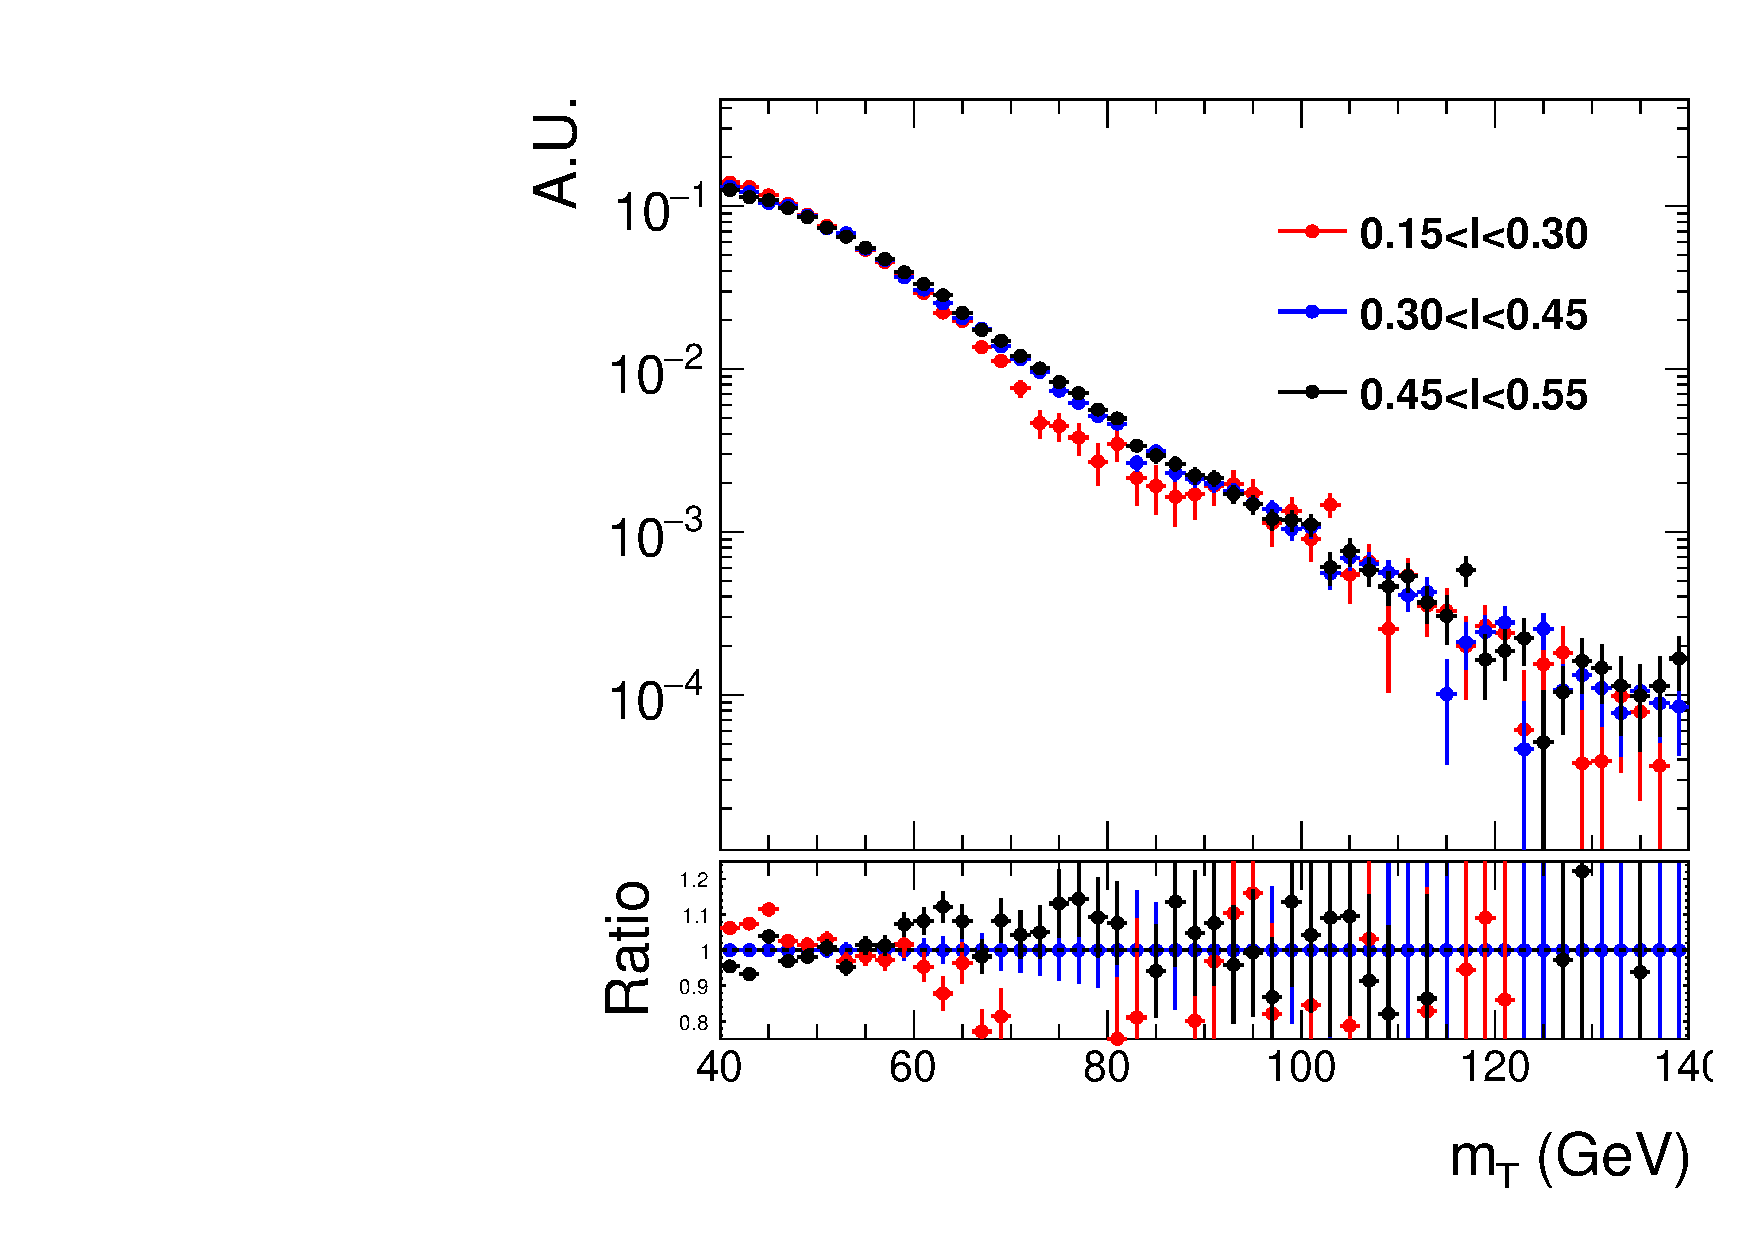
\includegraphics[width=0.49\textwidth]{plots/W/mt_qcd_shape_muon_wp.pdf}
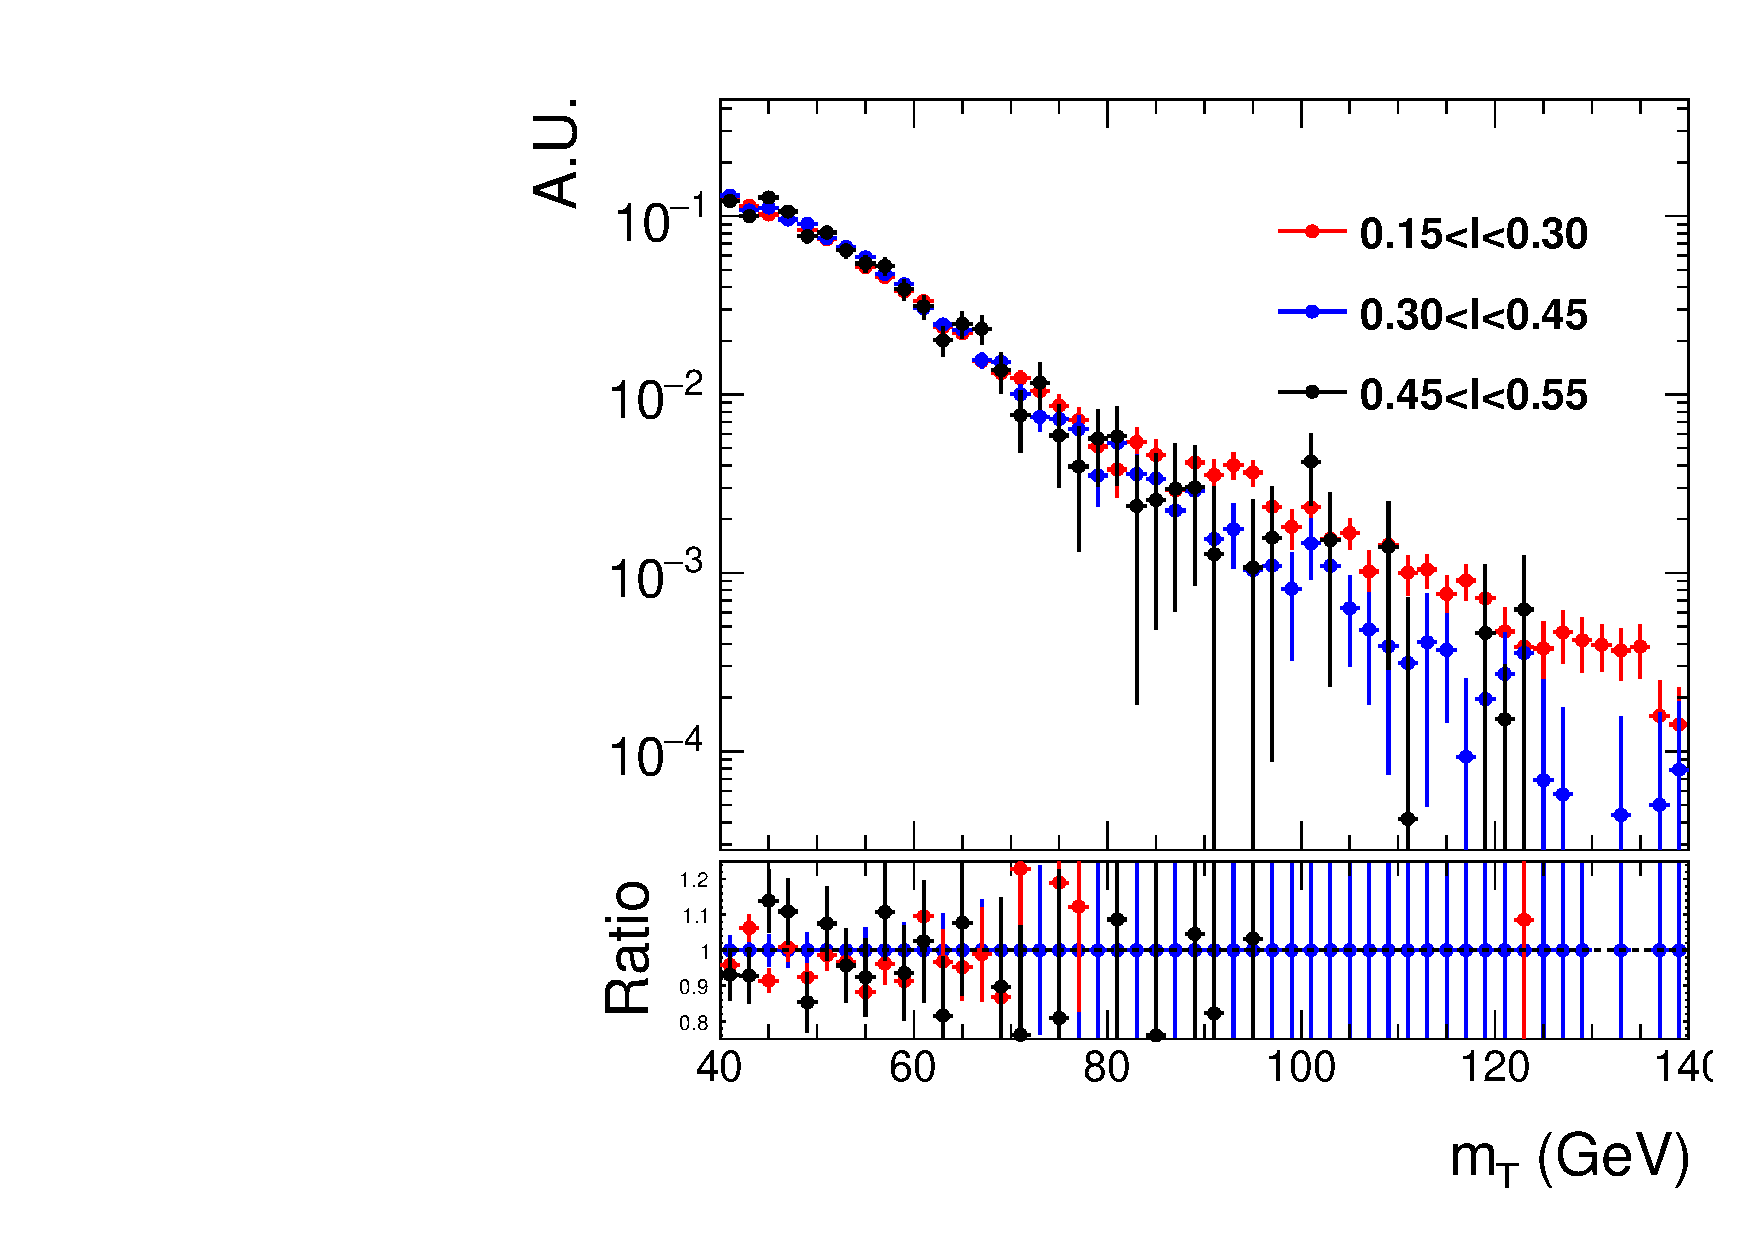
\includegraphics[width=0.49\textwidth]{plots/W/mt_qcd_shape_electron_wp.pdf}
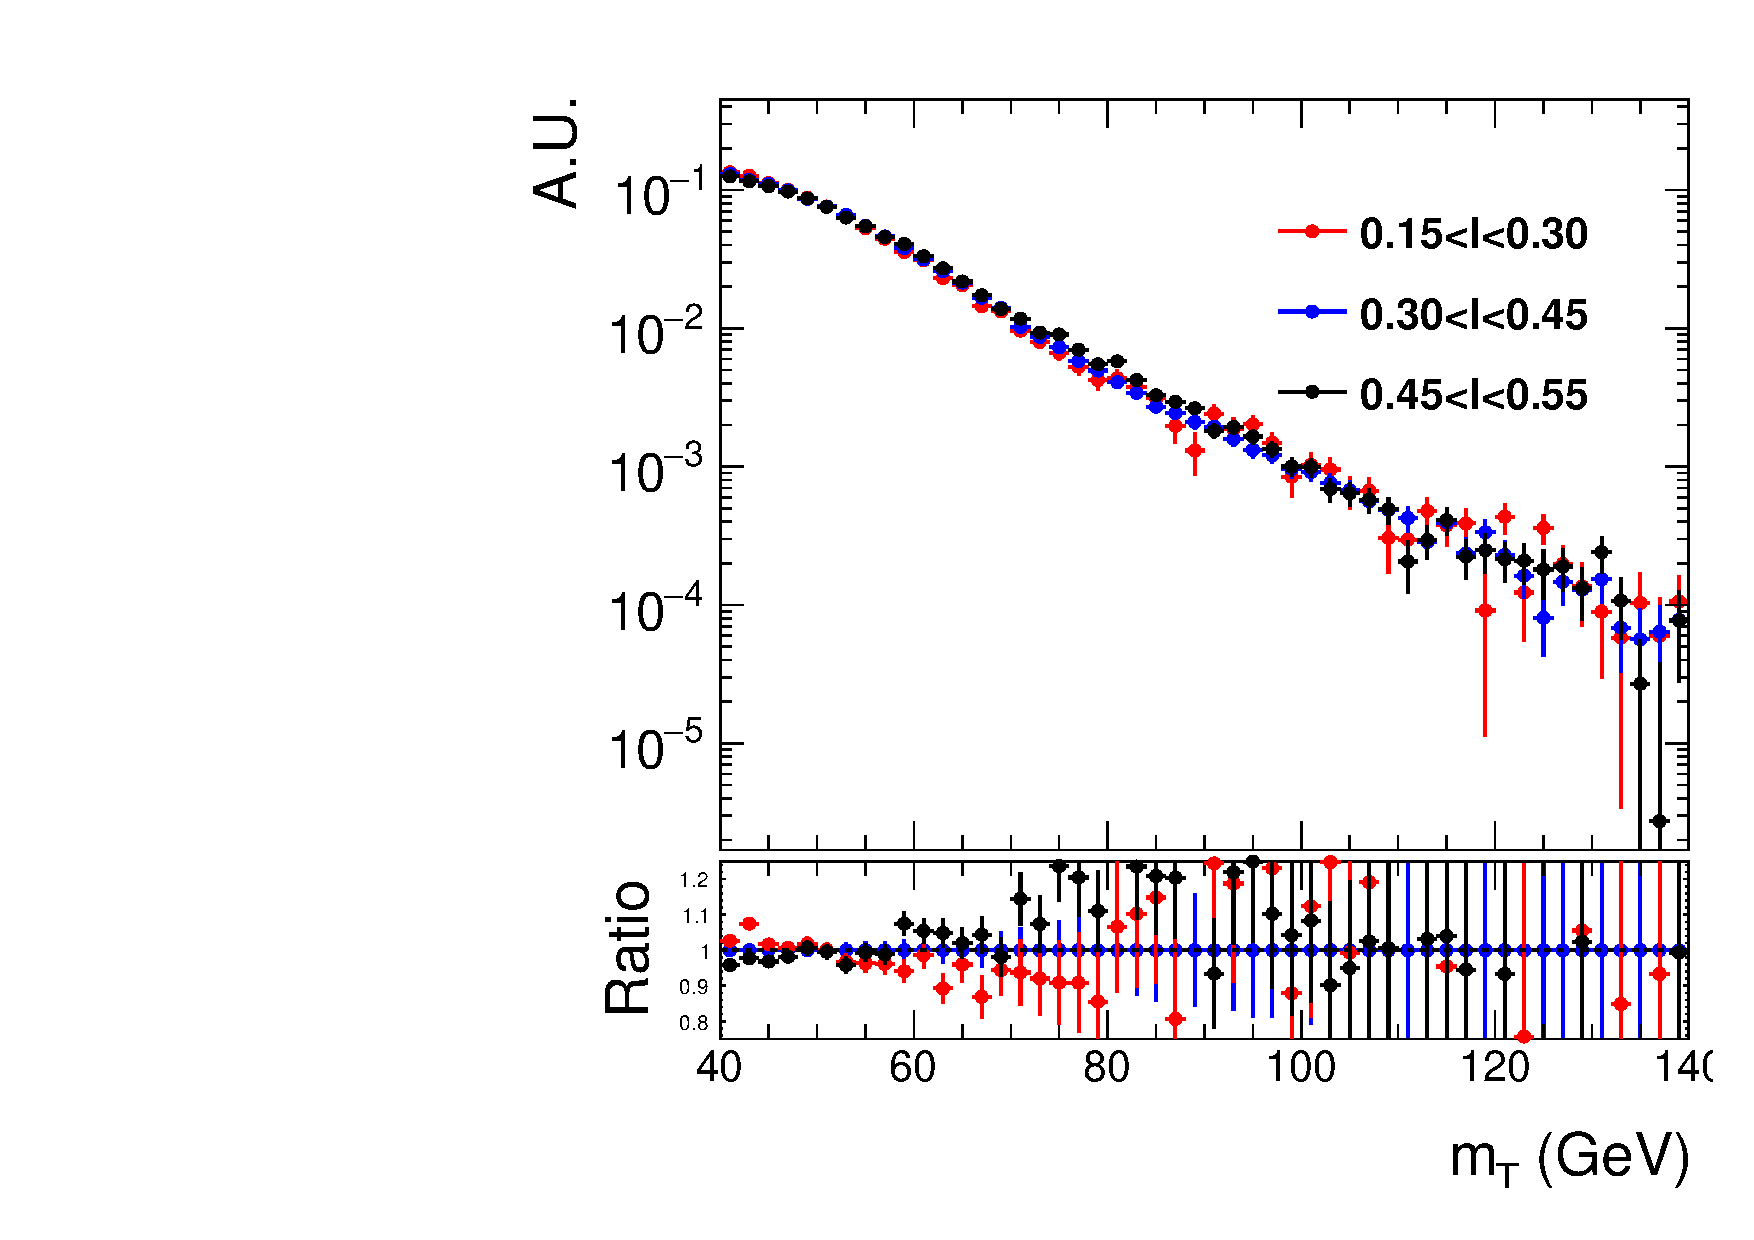
\includegraphics[width=0.49\textwidth]{plots/W/mt_qcd_shape_muon_wm.pdf}
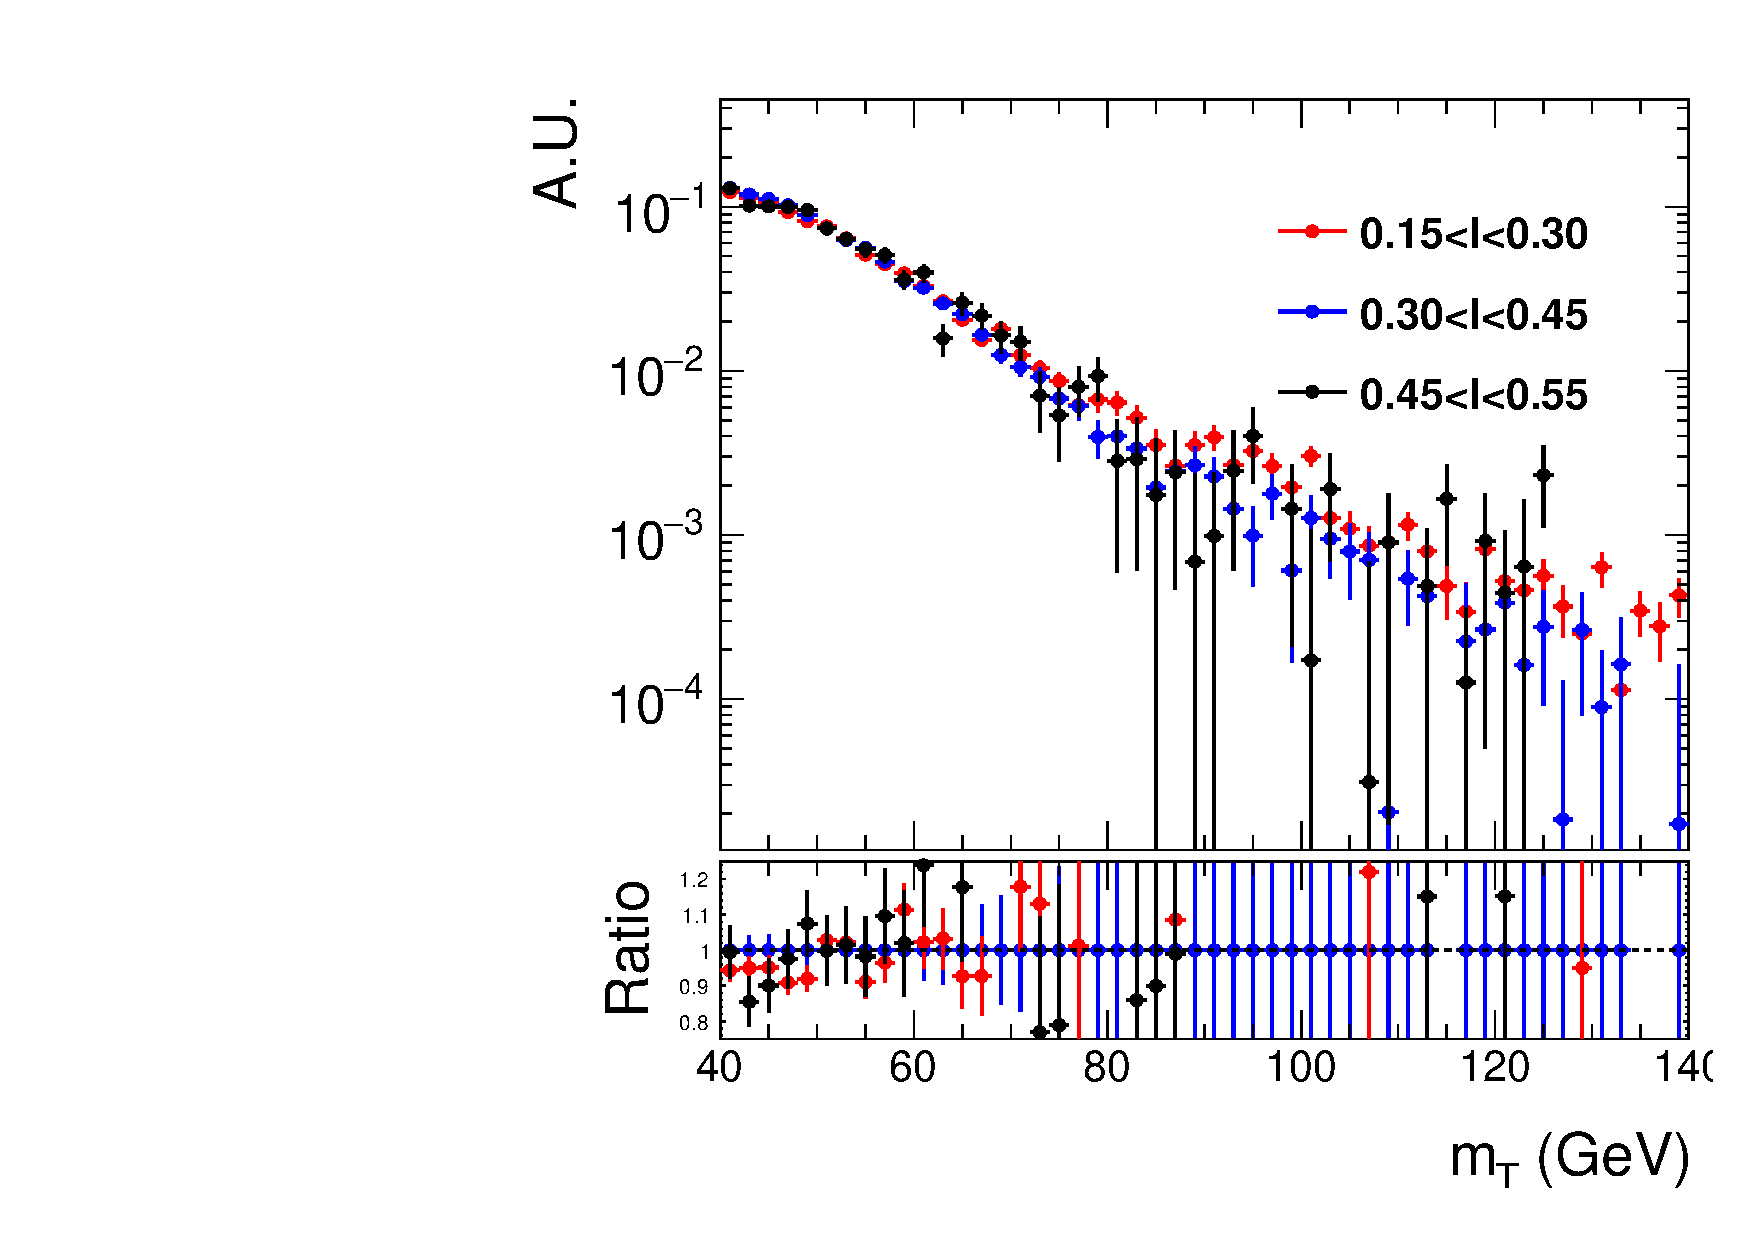
\includegraphics[width=0.49\textwidth]{plots/W/mt_qcd_shape_electron_wm.pdf}
\caption{QCD control regions for the muon (left) and electron (right) channels with positive  (top) and negative (bottom) charges.}
\label{fig:qcd:control}
\end{figure*}

\section{Uncertainties}\label{ch:unc}
Uncertainties in corrections are propagated to the final observable distributions \mt and \mll. These include variations on the lepton momentum scale factors, recoil corrections, prefiring probability, and lepton efficiency. Estimation of the uncertainties in each of these corrections is described in their respective chapters. This section summarizes how each of the uncertainties is propagated to the final discriminant distributions.
\subsubsection{\met Uncertainties}
Each uncertainty in \met modeling is an alternate set of recoil corrections which produces a variant on the \mt distribution. The difference between the baseline \mt distribution and each variant due to uncertainty in \met modeling is taken as the uncertainty. This is propagated into the final fit as a shape uncertainty by symmetrizing around the central \mt distribution. \met uncertainties are only applicable to the \W and \Z boson processes in the \Wp and \Wm boson signal channels. As described in Chapter~\ref{ch:recoil:unc}, there are a total of twelve uncertainty shapes from \met modeling---two due to model assumptions and ten due to each of the free parameters in each \pt bin fit. Each source of uncertainty is considered uncorrelated from the others.

\subsubsection{Lepton Efficiency Uncertainties}
Differences in lepton reconstruction and identification efficiency due to model and even selection choices are described in Chapter~\ref{ch:eff:systematics}. These uncertainties are applicable to all simulated processes in each of the \Wp, \Wm, and \Z boson channels. Each uncertainty is taken as the difference between \mll and \mt distributions with the baseline efficiency value and one of the variations. As with the \met uncertainties, these are symmetrized around the central value of \mll or \mt for each channel. Each source of uncertainty---MC generator, FSR model, background model, tag selection---is considered uncorrelated from the others.

\subsubsection{Lepton Momentum Uncertainties}
Uncertainties in lepton momentum scale factors are also propagated to \mll and \mt distributions. Differences between distributions constructed from the central value and $+1\sigma$ and $-1\sigma$ variations on the lepton momentum are taken as the uncertainty. 

\subsubsection{QCD shape uncertainty}
As described in the prior section, the QCD multijet background \mt distribution is estimated from data using non-isolated leptons in the range $0.30 < I < 0.45$. To account for differences in \mt distribution across varying levels of isolation, an uncertainty is taken as the difference between the \mt distributions in $0.30 < I < 0.45$ and $0.45 < I < 0.55$. As with the \met and efficiency scale factor uncertainties, the full uncertainty description is taken by symmetrizing around the central values from the $0.30 < I < 0.45$ region.  The QCD multijet uncertainty is considered uncorrelated between the \Wp and \Wm boson channels. 

\section{Summary}

The observed yields resulting from the signal extraction fits for all signal and background processes are listed in Table~\ref{tab:yield:ele:5} (Table~\ref{tab:yield:ele:13}) for the electron channels and Table~\ref{tab:yield:mu:5} (Table~\ref{tab:yield:mu:13}) for the muon channels at \sg (\sh). Quoted uncertainties include both statistical and systematic sources. The \Z boson \mll distributions are shown in Figure~\ref{fig:z:z:5} for \sg and Figure~\ref{fig:z:z:13} for \sh. The \mt distributions for the \W analyses are shown in Figure~\ref{fig:signal_wp} for \Wp and Figure~\ref{fig:signal_wm} for \Wm.

 
\begin{table}[htbp]
\centering
\newcolumntype{x}{D{,}{\,\pm\,}{3.3}}
\begin{tabular}{l@{\hspace*{1.5cm}}x{c}@{\hspace*{1.5cm}}x{c}@{\hspace*{1.5cm}}x}
Process   	      &   \multicolumn{1}{c}{\zee} &&  \multicolumn{1}{c}{\wep} &&  \multicolumn{1}{c}{\wem}  	    \\
%\cline{2-2}\cline{4-4}
\hline
Data                &   \multicolumn{1}{c}{$47734$}   && \multicolumn{1}{c}{$438547$}    && \multicolumn{1}{c}{$289179$}    \\
\hline
\hline
Signal                &   747323 , 862  &&    398952,  338    &&  252850 ,  274  \\    
QCD multijet          &   0 , 0   &&   27181 ,  333  &&  25968 ,  305  \\  
\ttbar             &   32 ,  3  &&    679 ,  11  &&  677 ,  11  \\    
Drell--Yan  	      &   508 ,  9  &&    11734 ,  176   &&  9684 ,  173  \\     
$\W \rightarrow \tau\nu$     &   < 1 &&    7372 ,  165    &&  5649 ,  159  \\    
Diboson               &   54 ,  5  &&    88 ,  1    &&  80 ,  1  \\    
\end{tabular}
\caption{Best-fit yields from various processes in \Z, \Wp, and \Wm boson with electron final states at \sg. Uncertainties shown are a combination of systematic and statistical.}
\label{tab:yield:ele:5}
\end{table}



\begin{table}[htbp]
\centering
\newcolumntype{x}{D{,}{\,\pm\,}{3.3}}
\begin{tabular}{l@{\hspace*{1.5cm}}x{c}@{\hspace*{1.5cm}}x{c}@{\hspace*{1.5cm}}x}
Process   	      &   \multicolumn{1}{c}{\zmm} &&  \multicolumn{1}{c}{\wmp} &&  \multicolumn{1}{c}{\wmm}  	    \\
%\cline{2-2}\cline{4-4}
\hline
Data                &   \multicolumn{1}{c}{$79345$}   && \multicolumn{1}{c}{$672817$}    && \multicolumn{1}{c}{$428156$}    \\
\hline
\hline
Signal                &   79076 ,  249  &&    626189,  554    &&  389637 ,  420  \\    
QCD multijet          &   0 , 0   &&   12496 ,  238  &&  12616 ,  162  \\  
\ttbar             &   49 ,  5  &&    828 ,  13  &&  836 ,  14  \\    
Drell--Yan  	      &   126 ,  3  &&    33295 ,  258   &&  25066 ,  194  \\     
$\W \rightarrow \tau\nu$     &   < 1 &&    13268 ,  232    &&  8450 ,  159  \\    
Diboson               &   88 ,  9  &&    125 ,  2    &&  112 ,  2  \\    
\end{tabular}
\caption{Best-fit yields from various processes in \Z, \Wp, and \Wm bosons with muon final states at \sg. Uncertainties shown are a combination of systematic and statistical.}
\label{tab:yield:mu:5}
\end{table}

\begin{table}[htbp]
\centering
\newcolumntype{x}{D{,}{\,\pm\,}{3.3}}
\begin{tabular}{l@{\hspace*{1.5cm}}x{c}@{\hspace*{1.5cm}}x{c}@{\hspace*{1.5cm}}x}
Process   	      &   \multicolumn{1}{c}{\zee} &&  \multicolumn{1}{c}{\wep} &&  \multicolumn{1}{c}{\wem}  	    \\
%\cline{2-2}\cline{4-4}
\hline
Data                &   \multicolumn{1}{c}{$76229$}   && \multicolumn{1}{c}{$709630$}    && \multicolumn{1}{c}{$578135$}    \\
\hline
\hline
Signal                &   73800 ,  1320  &&    605443,  372    &&  477096 ,  342  \\    
QCD multijet          &   0 , 0    &&     77133 ,  475  &&  76496 ,  442  \\  
\ttbar             &   203 ,  21  &&    5833 ,  94  &&  5871 ,  94  \\    
Drell--Yan  	      &   748 ,  14  &&    21222 ,  167   &&  18653 ,  153  \\     
$\W \rightarrow \tau\nu$     &   < 1 &&    9434 ,  109    &&  7422 ,  93  \\    
Diboson               &   93 ,  9  &&    240 ,  3    &&  231 ,  3  \\    
\end{tabular}
\caption{Best-fit yields from various processes in \Z, \Wp, and \Wm bosons with electron final states at \sh. Uncertainties shown are a combination of systematic and statistical.[estimating QCD yield for Z with e-mu selection, will add to table]}
\label{tab:yield:ele:13}
\end{table}


\begin{table}[htbp]
\centering
\newcolumntype{x}{D{,}{\,\pm\,}{3.3}}
\begin{tabular}{l@{\hspace*{1.5cm}}x{c}@{\hspace*{1.5cm}}x{c}@{\hspace*{1.5cm}}x}
Process   	      &   \multicolumn{1}{c}{\zmm} &&  \multicolumn{1}{c}{\wmp} &&  \multicolumn{1}{c}{\wmm}  	    \\
%\cline{2-2}\cline{4-4}
\hline
Data                &   \multicolumn{1}{c}{$128713$}   && \multicolumn{1}{c}{$1014670$}    && \multicolumn{1}{c}{$795518$}    \\
\hline
\hline
Signal                &   126473 ,  2261  &&    902641,  666    &&  696182 ,  586  \\    
QCD multijet          &   0 , 0    &&   50374 , 337  &&  46450 ,  315  \\  
\ttbar             &   326 ,  34  &&    6558 ,  100  &&  6148 ,  89  \\    
Drell--Yan  	      &   204 ,  4  &&    55084 ,  305   &&  46742 ,  241  \\     
$\W \rightarrow \tau\nu$     &   < 1  &&    17802 ,  229    &&  14285 ,  170  \\    
Diboson               &   151 ,  15  &&    317 ,  4    &&  296 ,  4  \\    
\end{tabular}
\caption{Best-fit yields from various processes in \Z, \Wp, and \Wm bosons with muon final states at \sh. Uncertainties shown are a combination of systematic and statistical[estimating QCD yield for Z with e-mu selection, will add to table].}
\label{tab:yield:mu:13}
\end{table}

\begin{figure}
\centering
\begin{subfigure}{.50\textwidth}
\centering
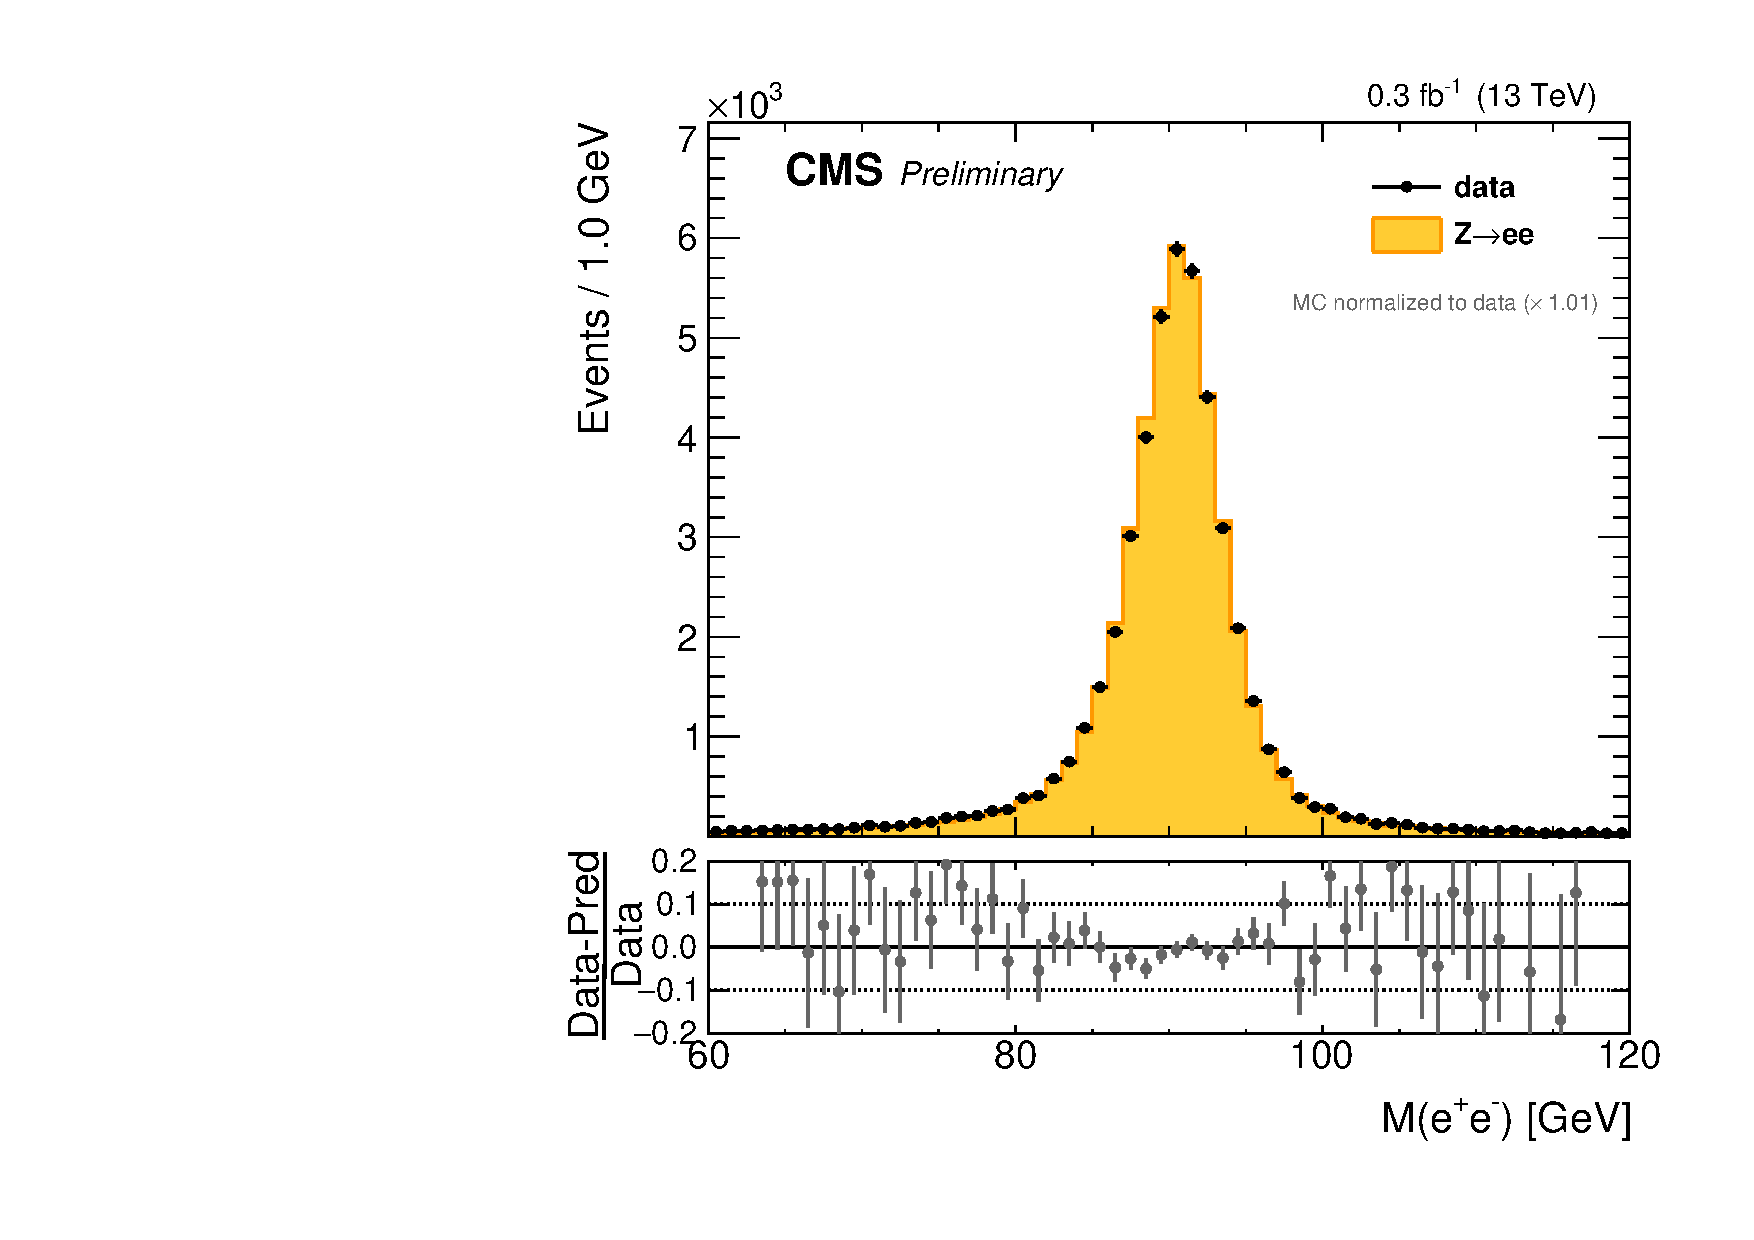
\includegraphics[width=\linewidth]{plots/Z/5tev/zee_norm.pdf}
\end{subfigure}%
\centering
\begin{subfigure}{.50\textwidth}
\centering
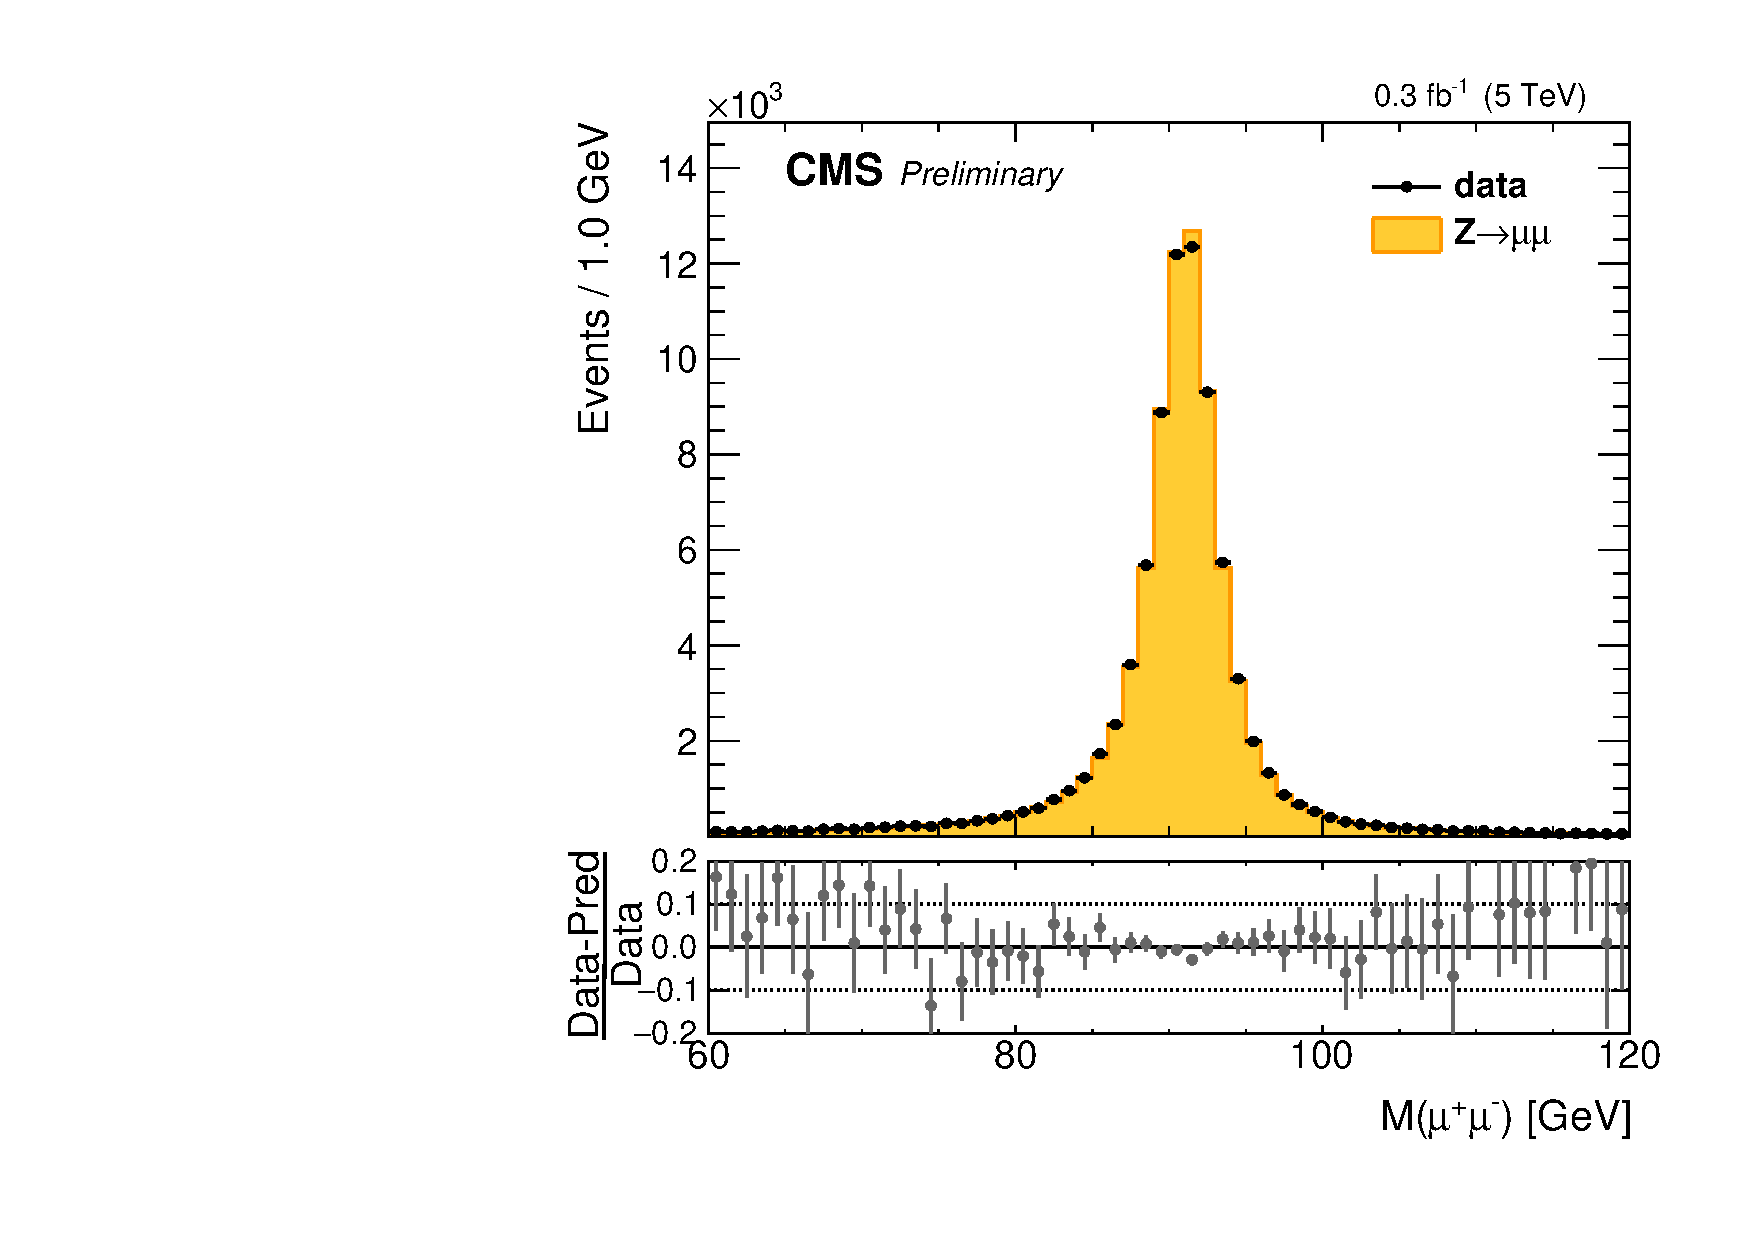
\includegraphics[width=\linewidth]{plots/Z/5tev/zmm.pdf}
\end{subfigure}%
\\
\centering
\begin{subfigure}{.50\textwidth}
\centering
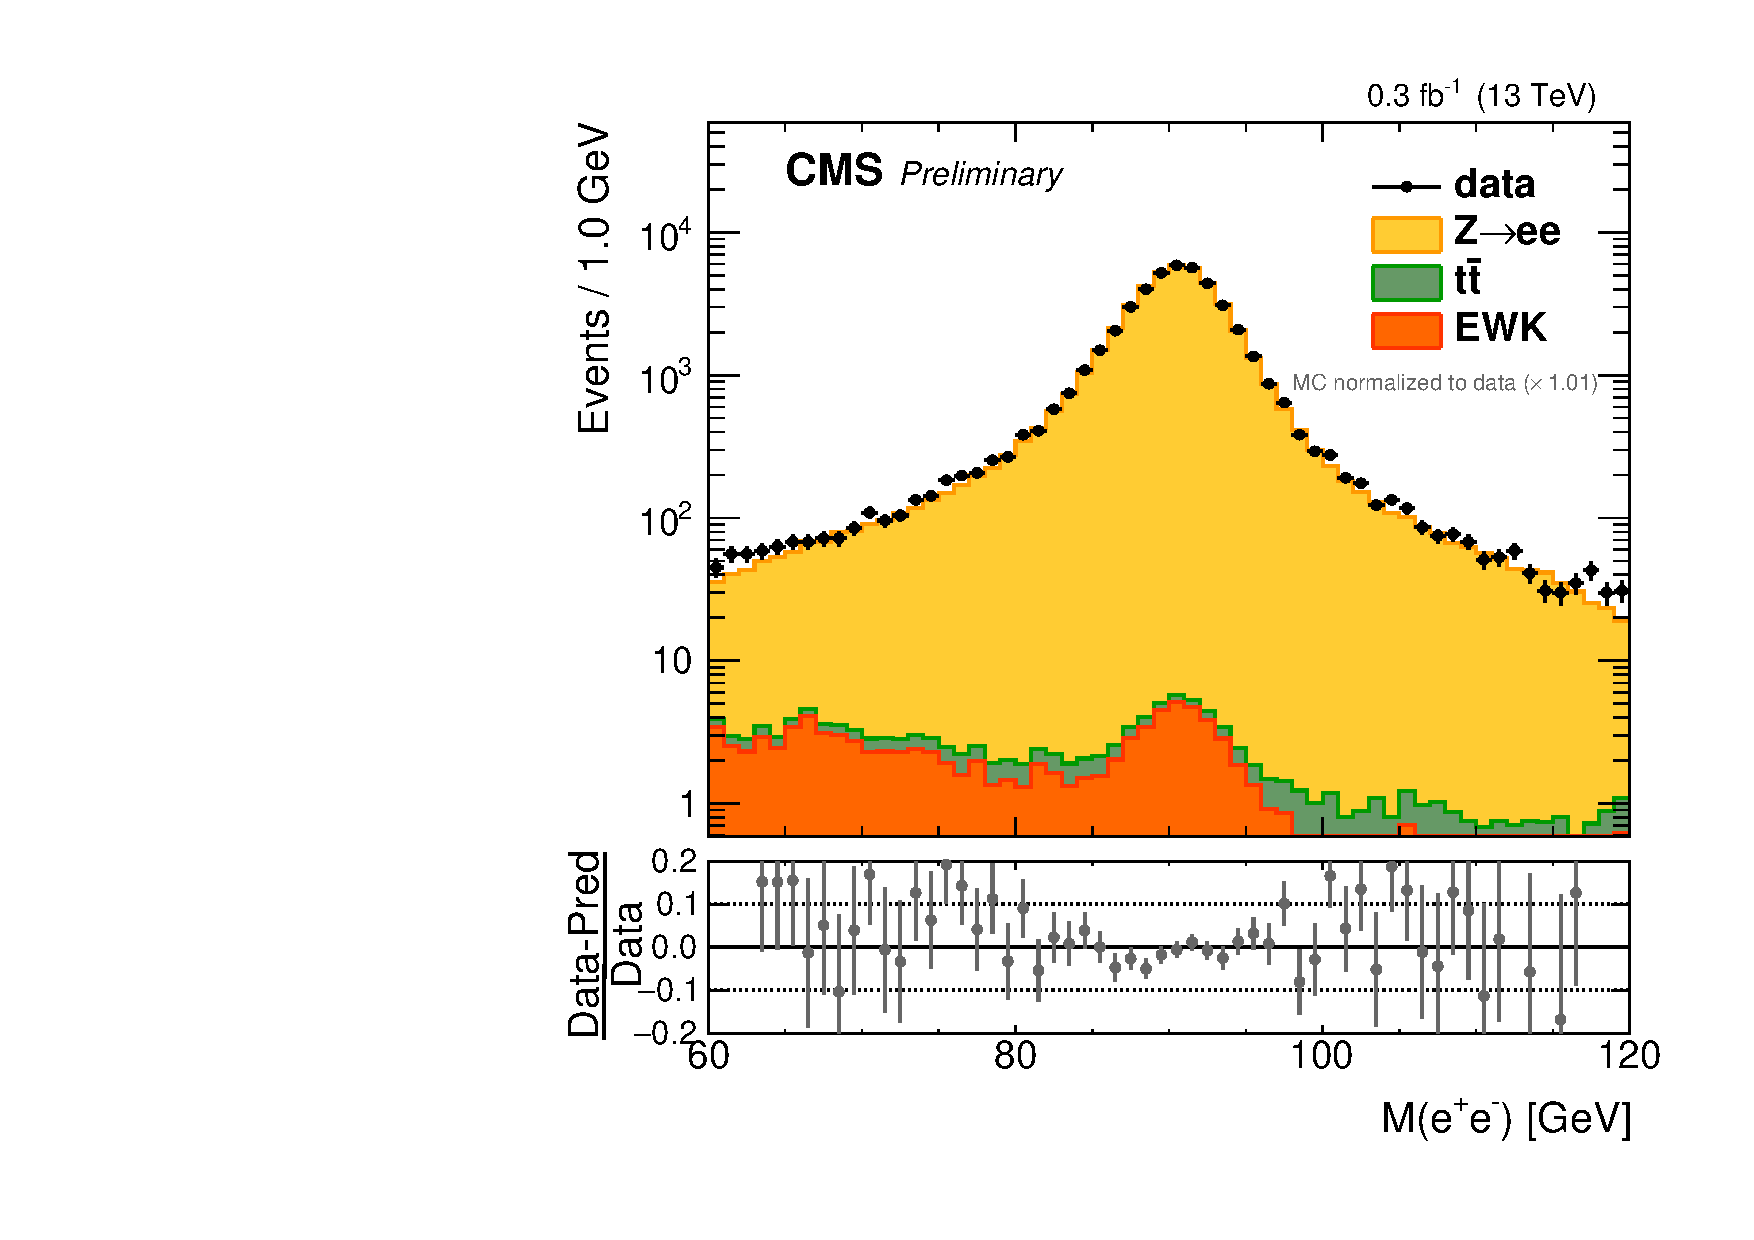
\includegraphics[width=\linewidth]{plots/Z/5tev/zeelog_norm.pdf}
\end{subfigure}%
\centering
\begin{subfigure}{.50\textwidth}
\centering
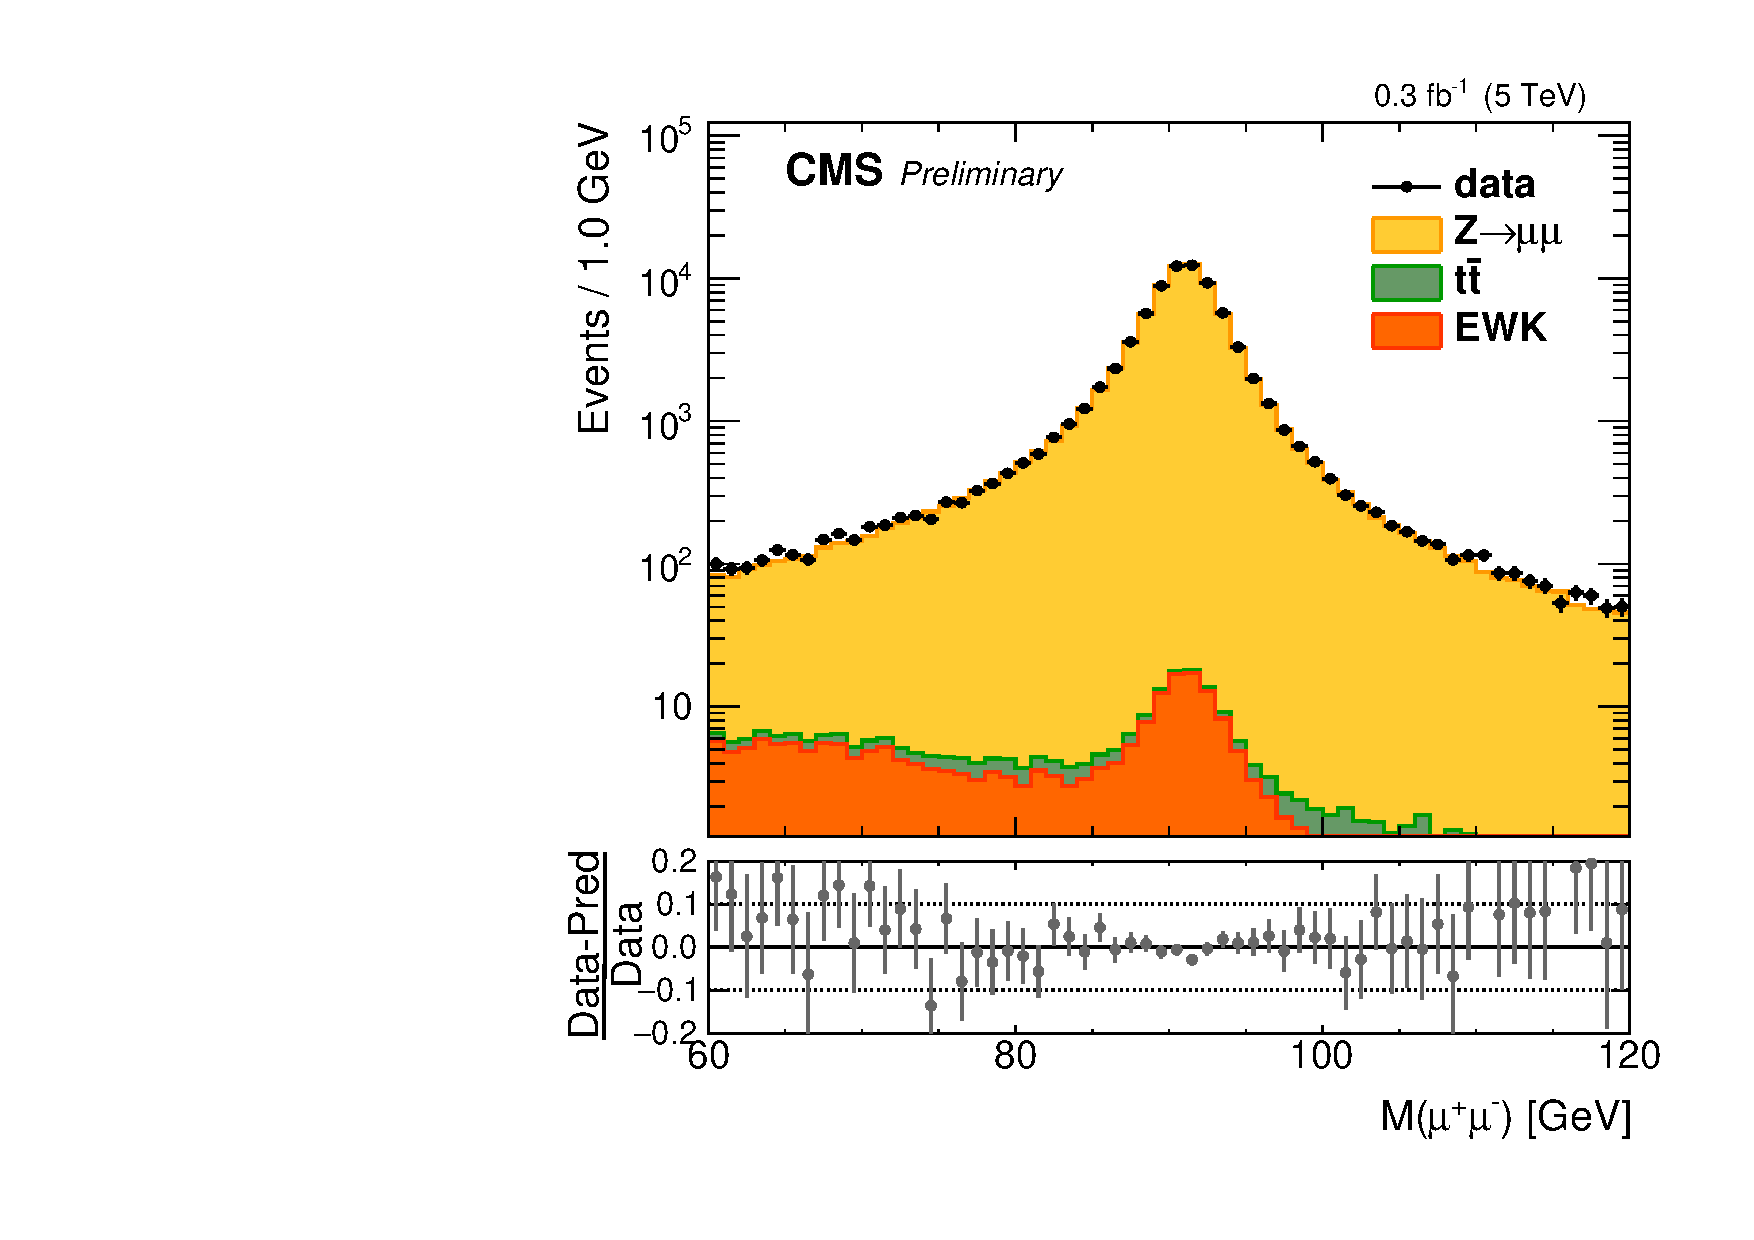
\includegraphics[width=\linewidth]{plots/Z/5tev/zmmlog.pdf}
\end{subfigure}%
\caption{The \mll distributions for \zee (left) and \zmm (right) at \sg. The simulated events have been normalized to data.}
\label{fig:z:z:5}
\end{figure}

\begin{figure}
\centering
\begin{subfigure}{.50\textwidth}
\centering
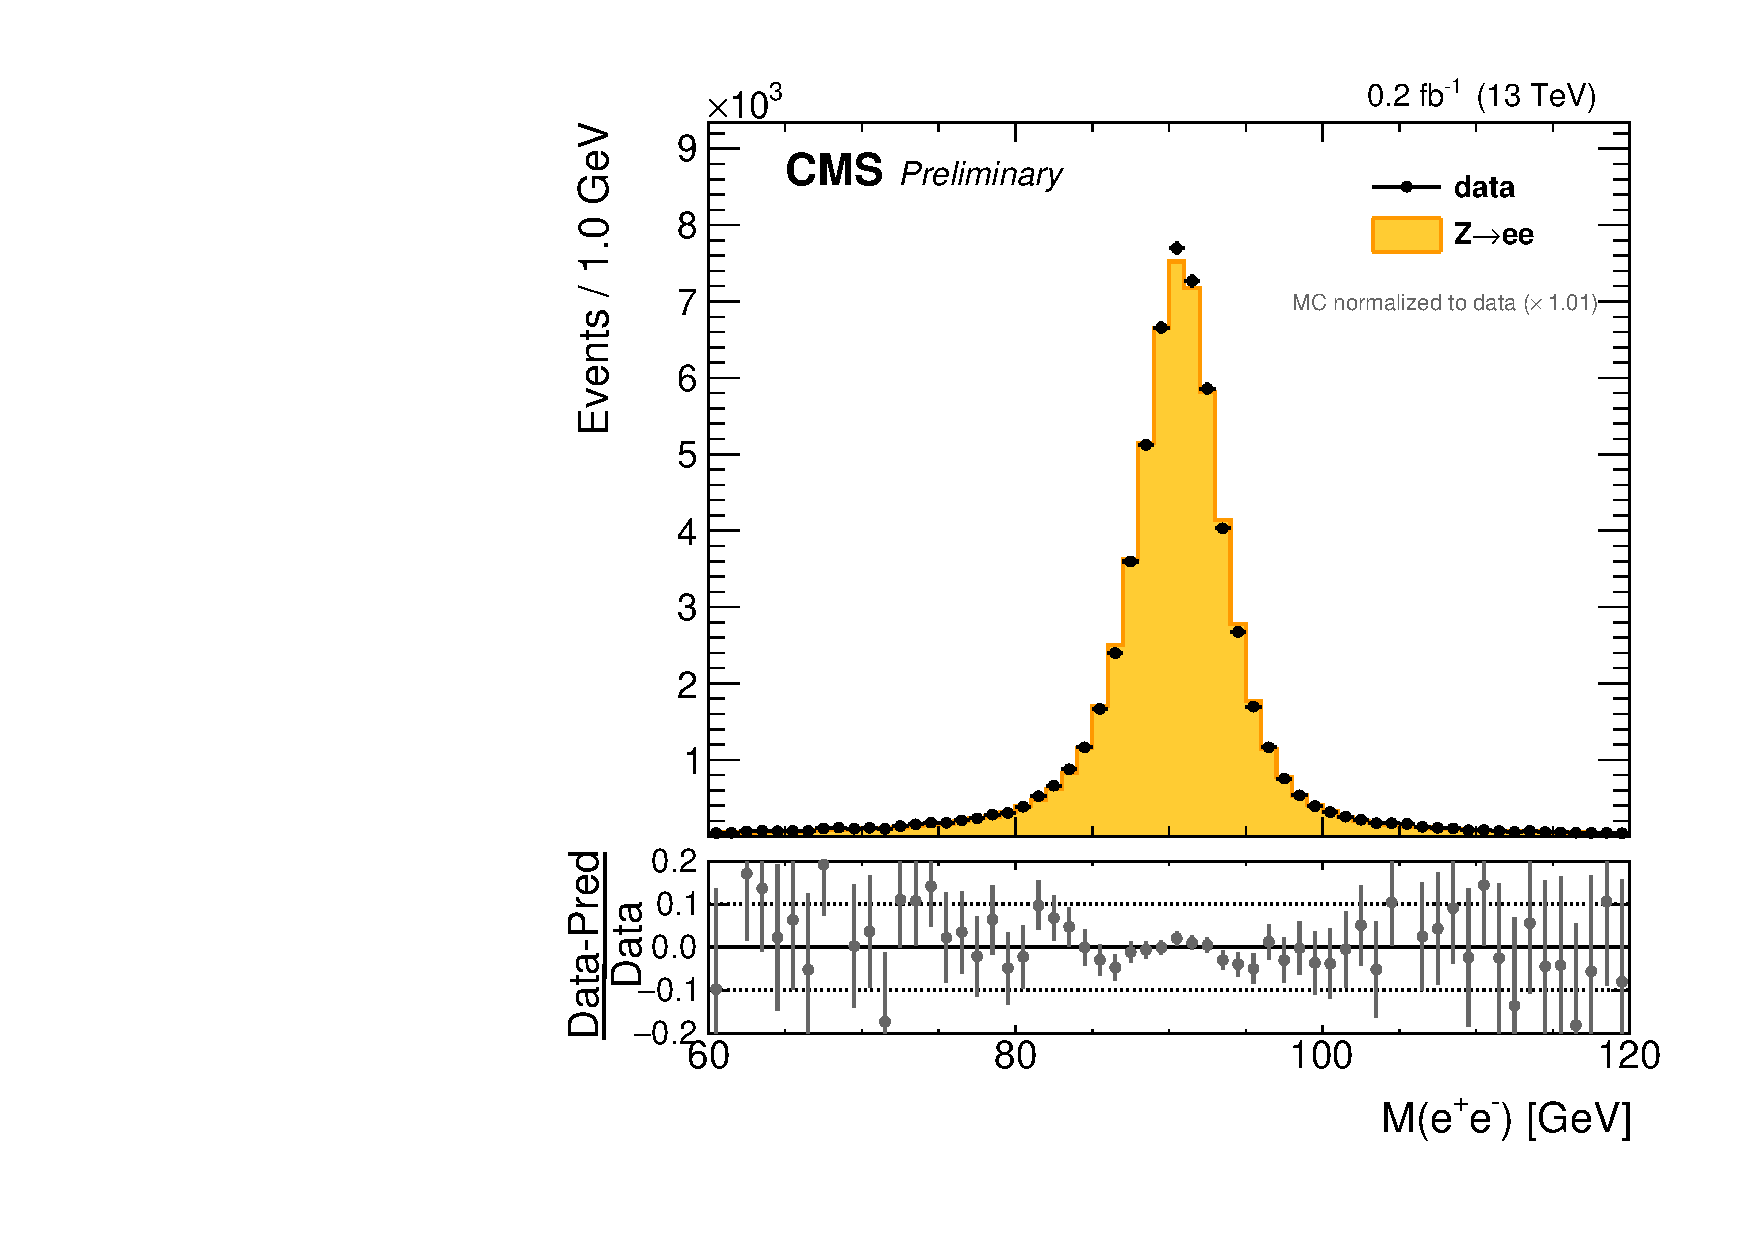
\includegraphics[width=\linewidth]{plots/Z/13tev/zee_norm.pdf}
\end{subfigure}%
\centering
\begin{subfigure}{.50\textwidth}
\centering
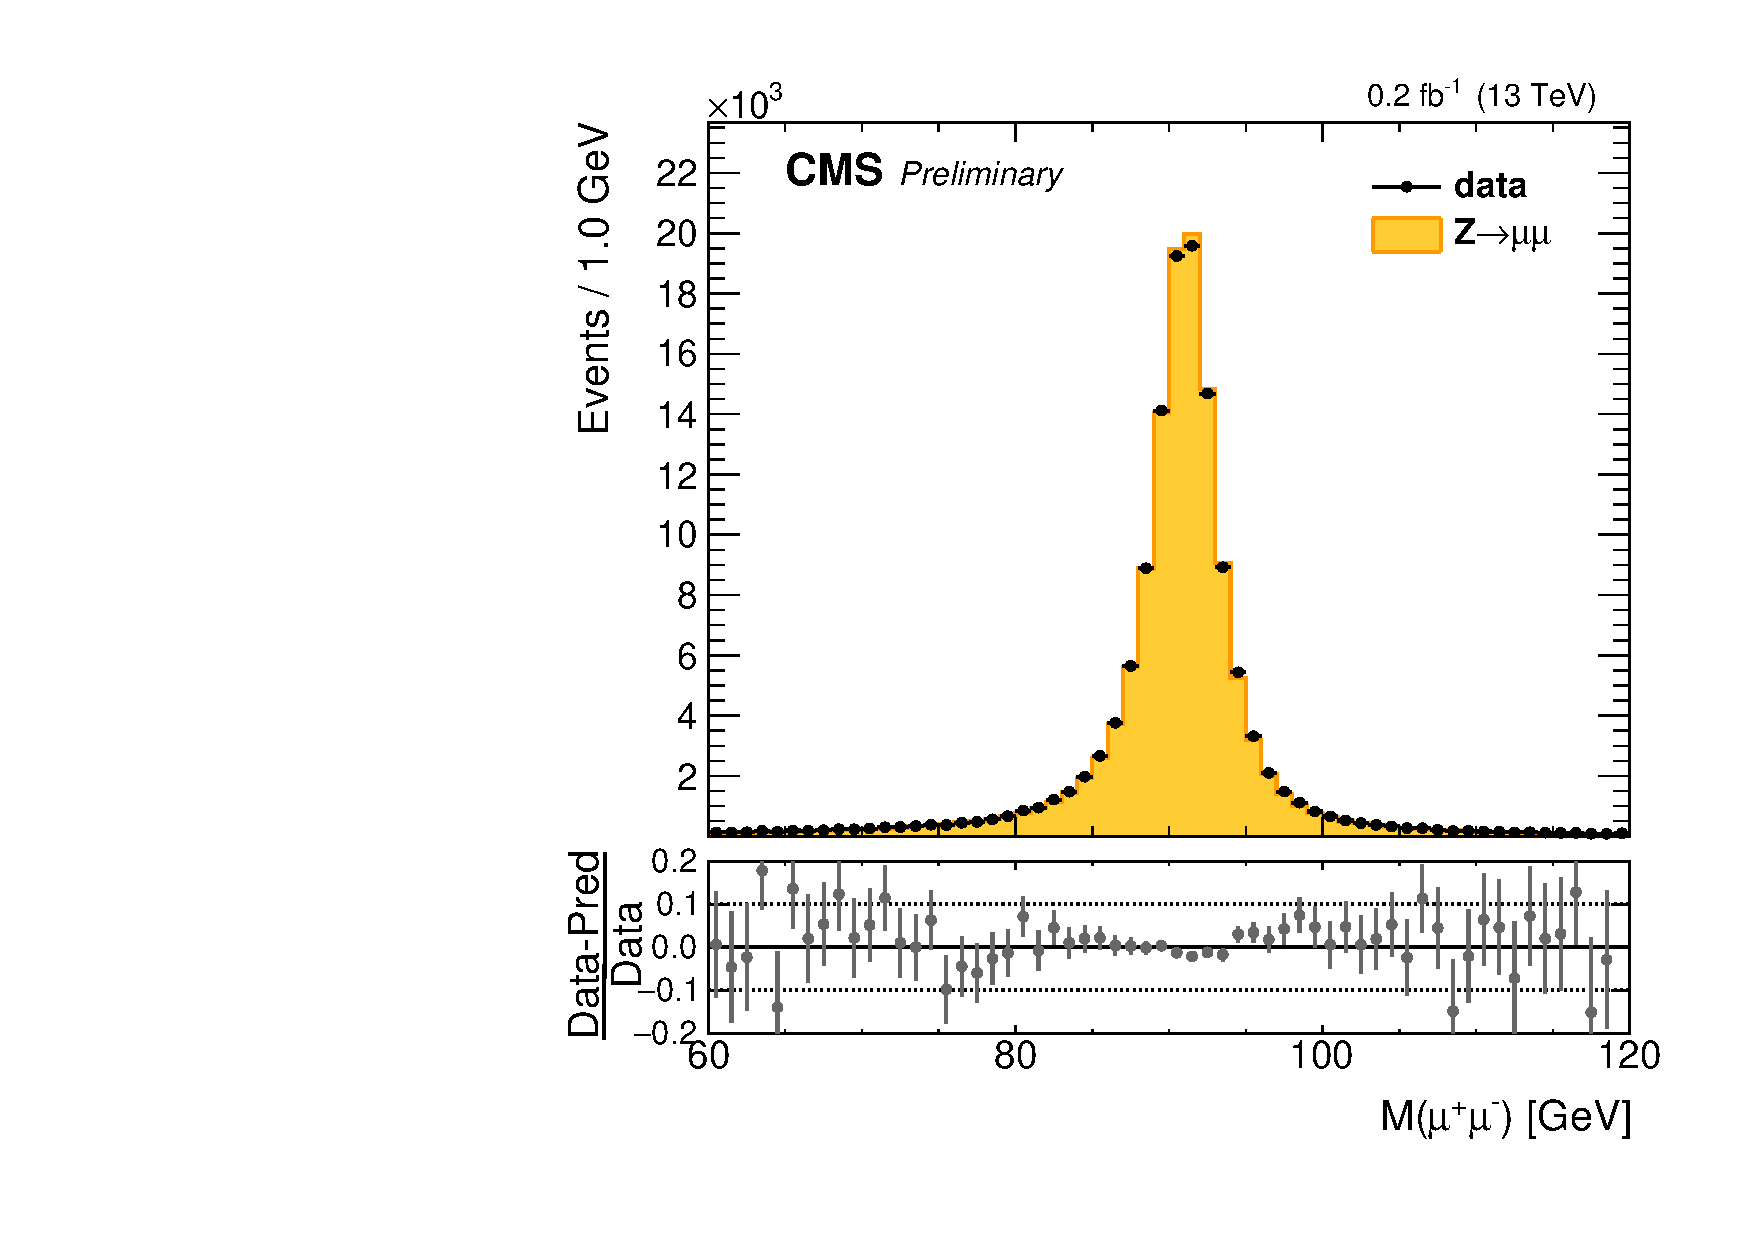
\includegraphics[width=\linewidth]{plots/Z/13tev/zmm.pdf}
\end{subfigure}%
\\
\centering
\begin{subfigure}{.50\textwidth}
\centering
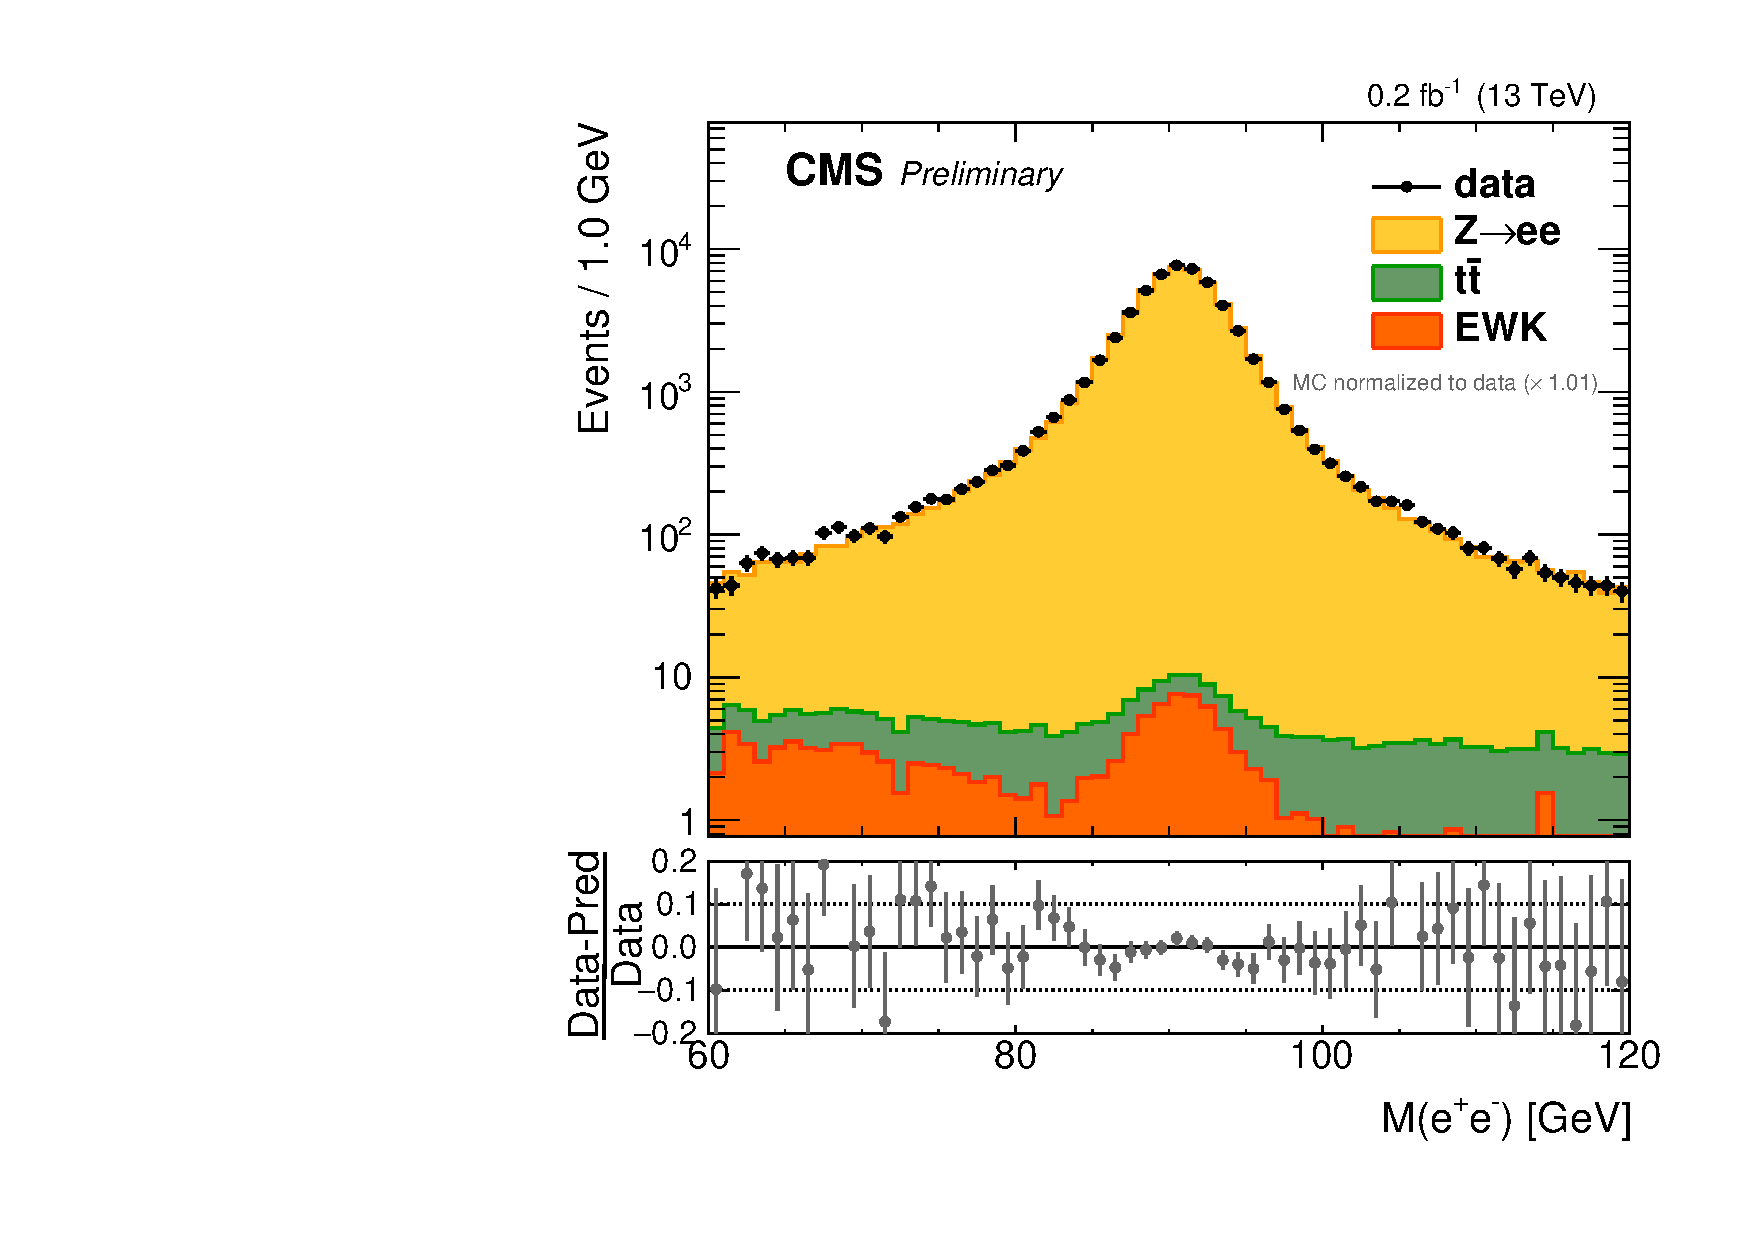
\includegraphics[width=\linewidth]{plots/Z/13tev/zeelog_norm.pdf}
\end{subfigure}%
\centering
\begin{subfigure}{.50\textwidth}
\centering
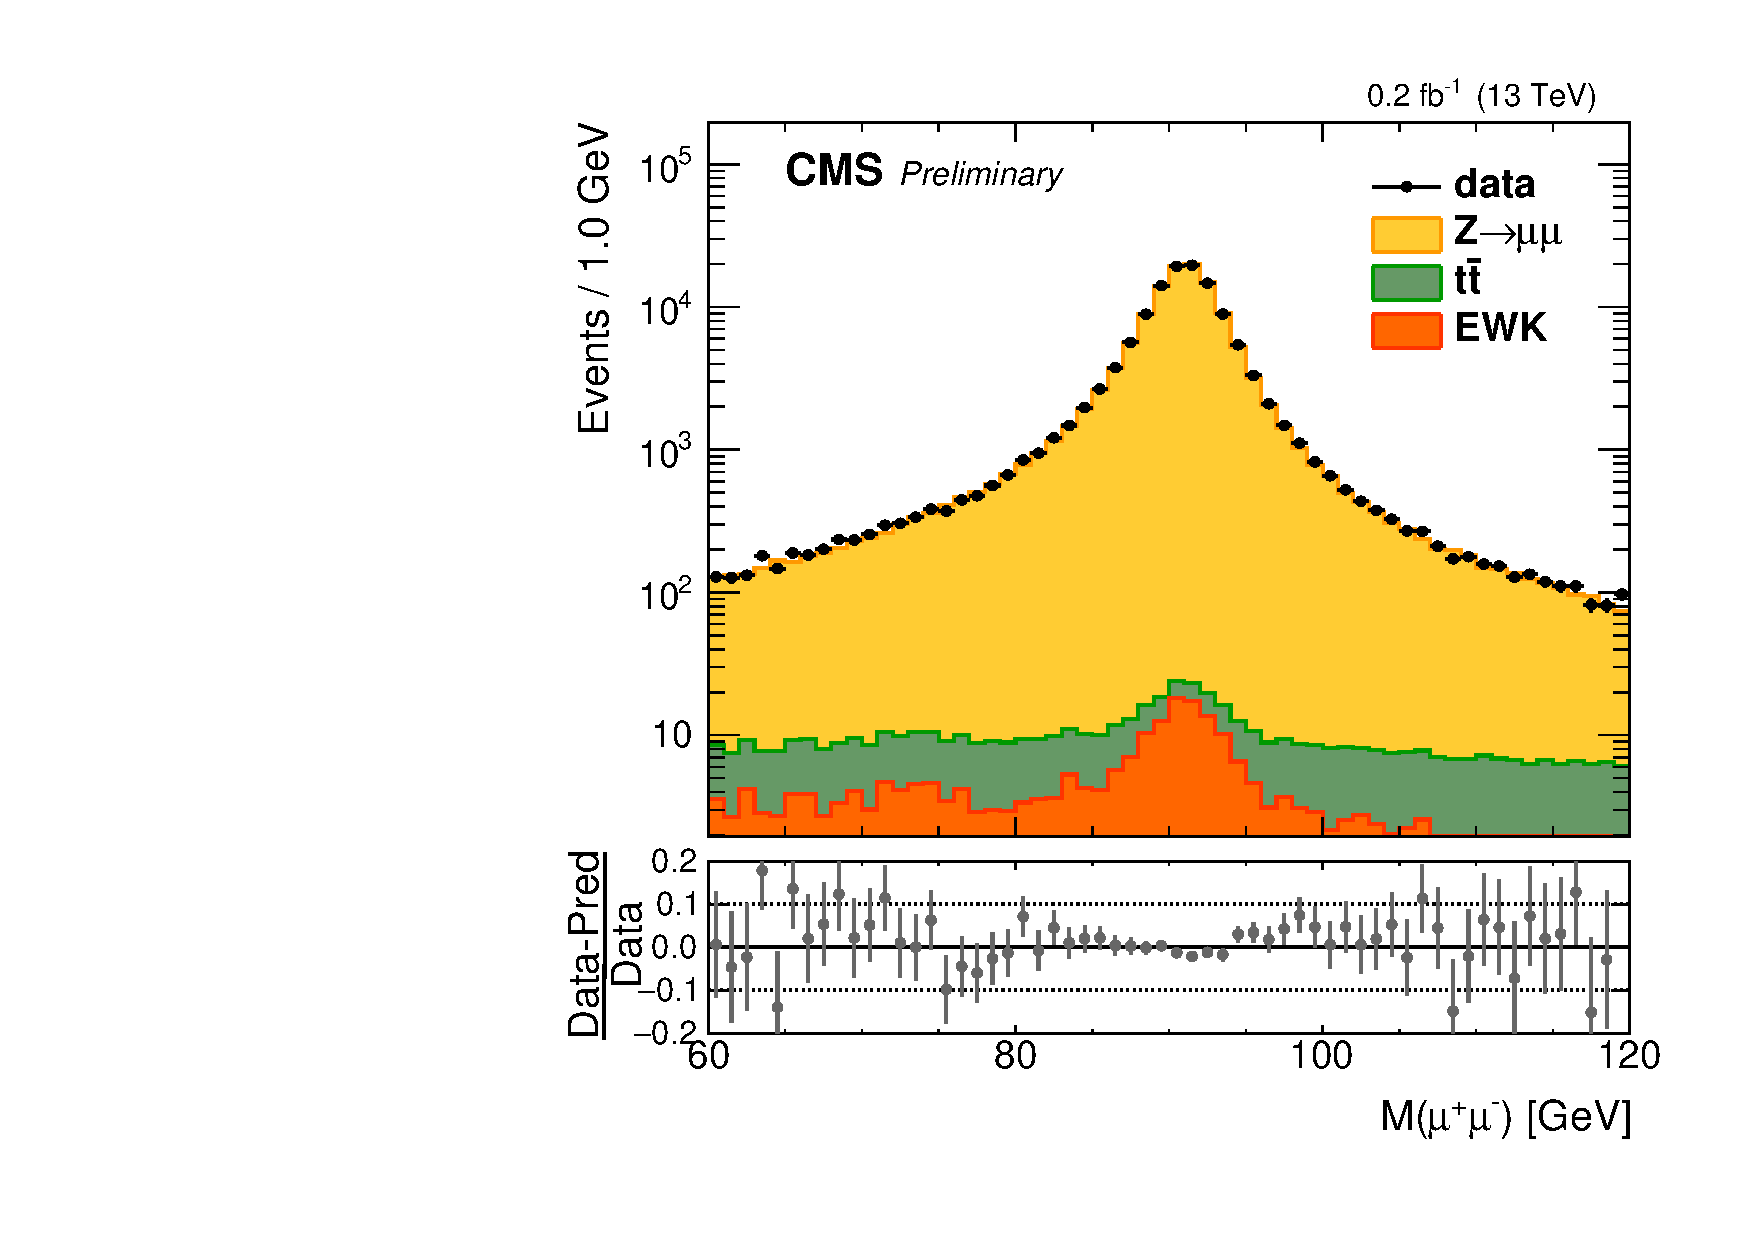
\includegraphics[width=\linewidth]{plots/Z/13tev/zmmlog.pdf}
\end{subfigure}%
\caption{The \mll distributions for \zee (left) and \zmm (right) at \sh. The simulated events have been normalized to data.}
\label{fig:z:z:13}
\end{figure}

\begin{figure*}[htb]
\centering
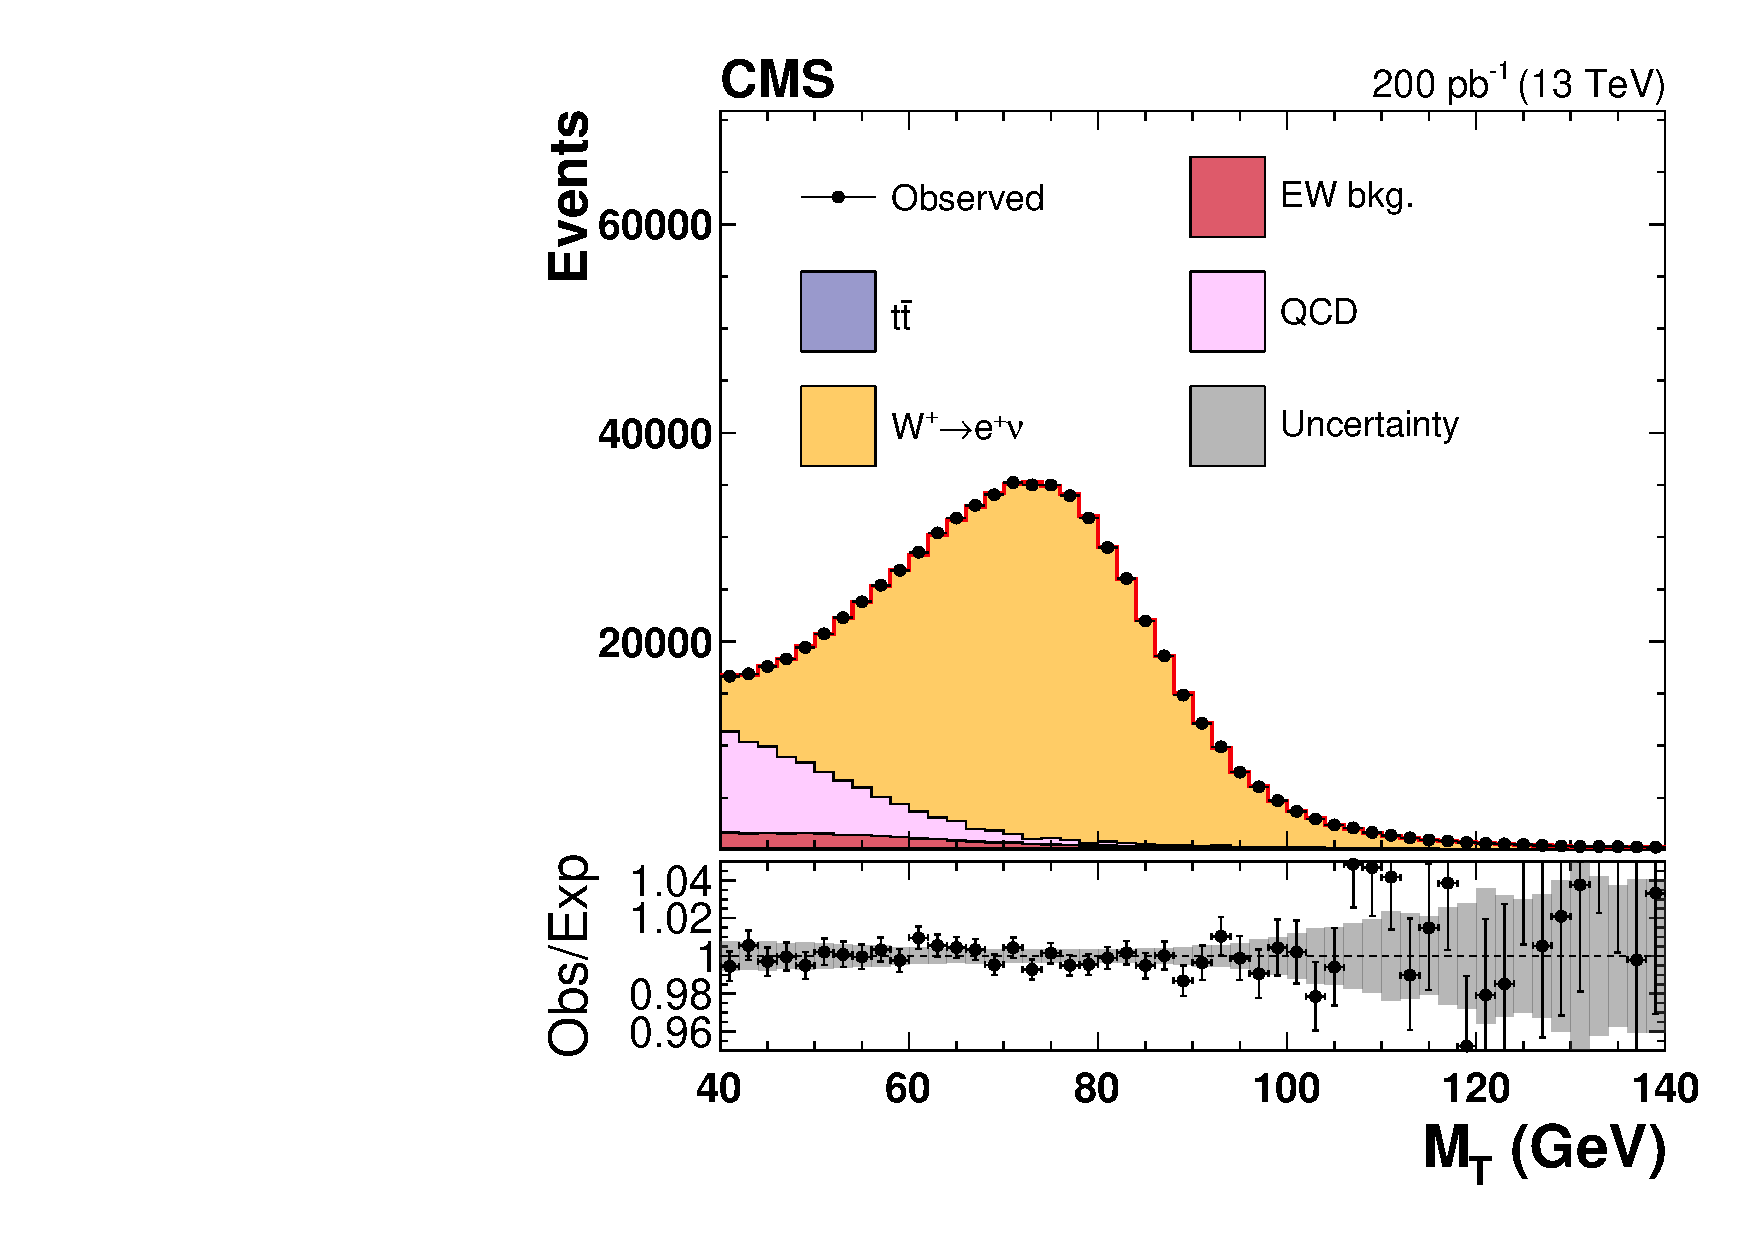
\includegraphics[width=0.49\textwidth]{plots/W/wpefit13.pdf}
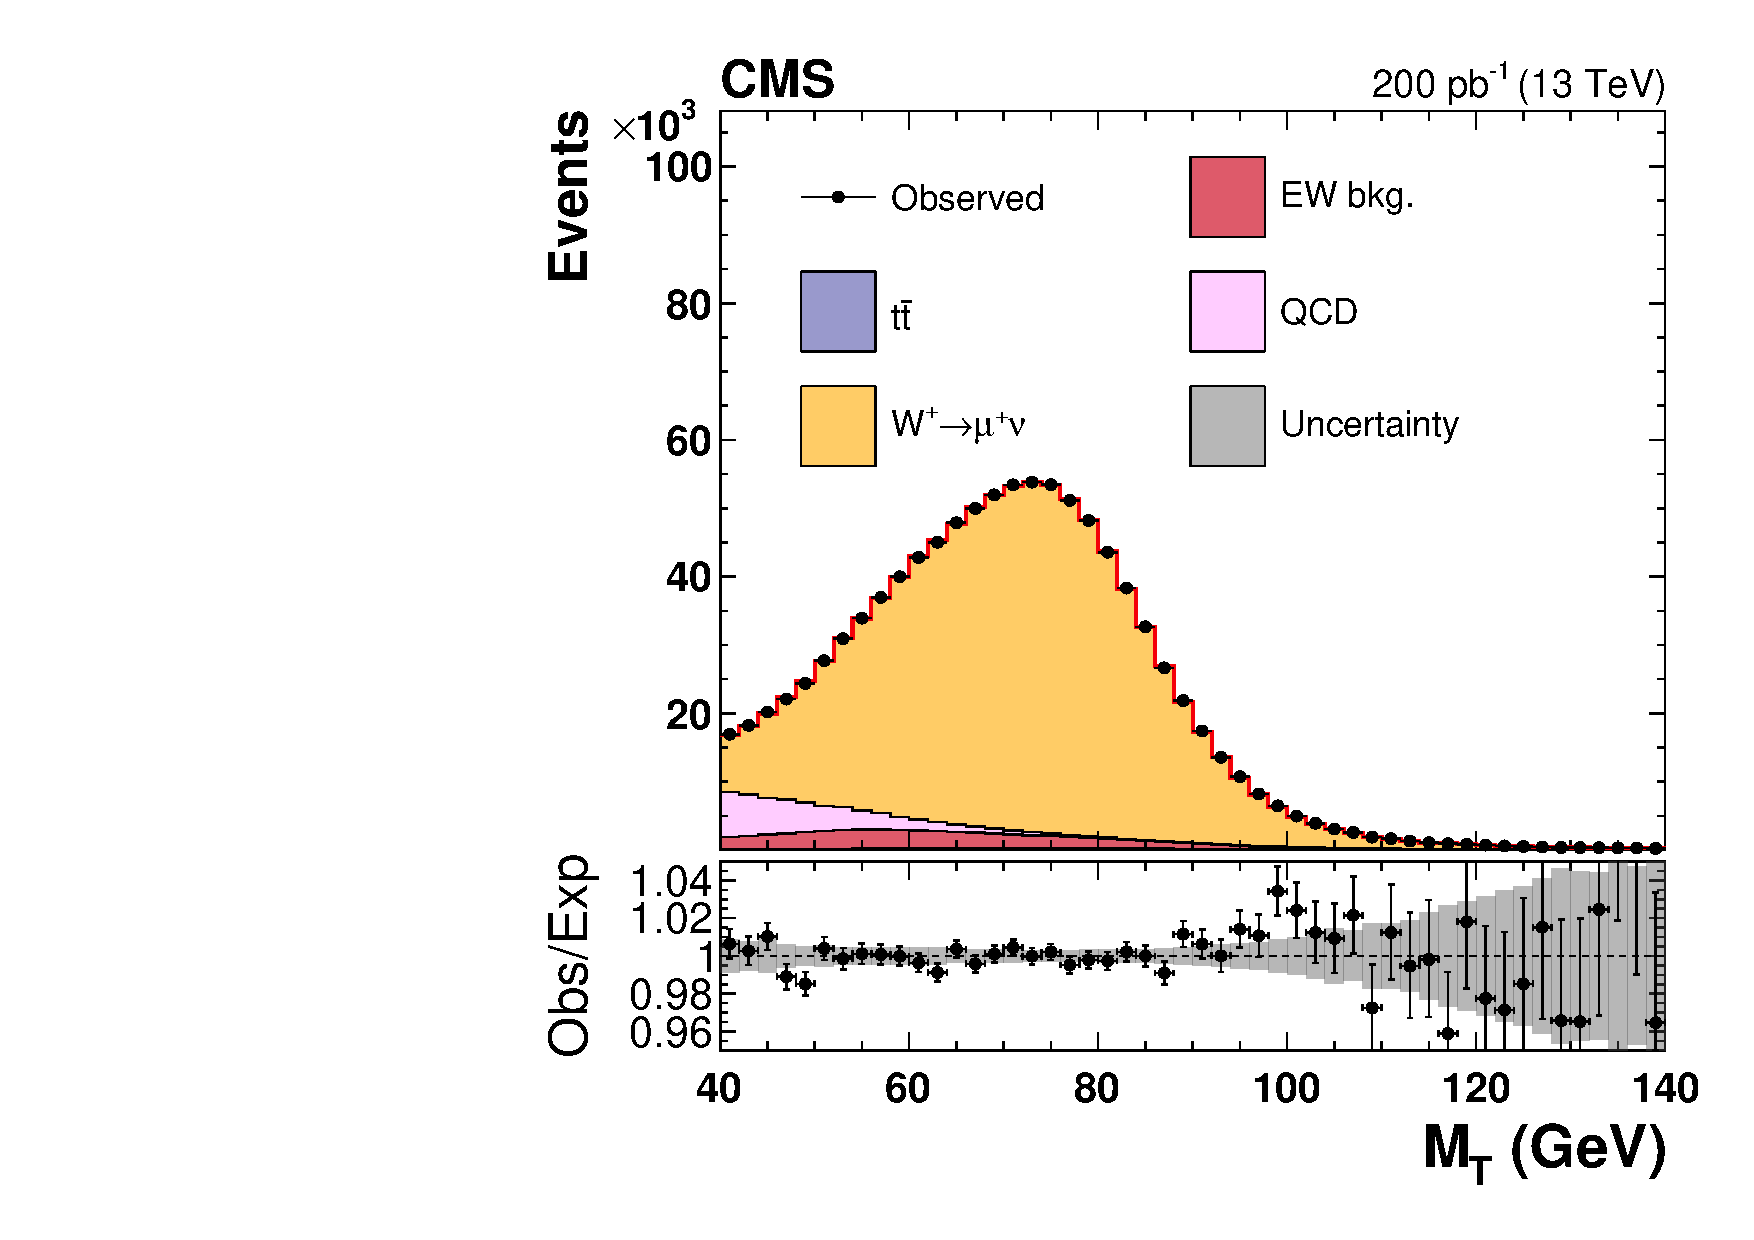
\includegraphics[width=0.49\textwidth]{plots/W/wpmfit13.pdf}
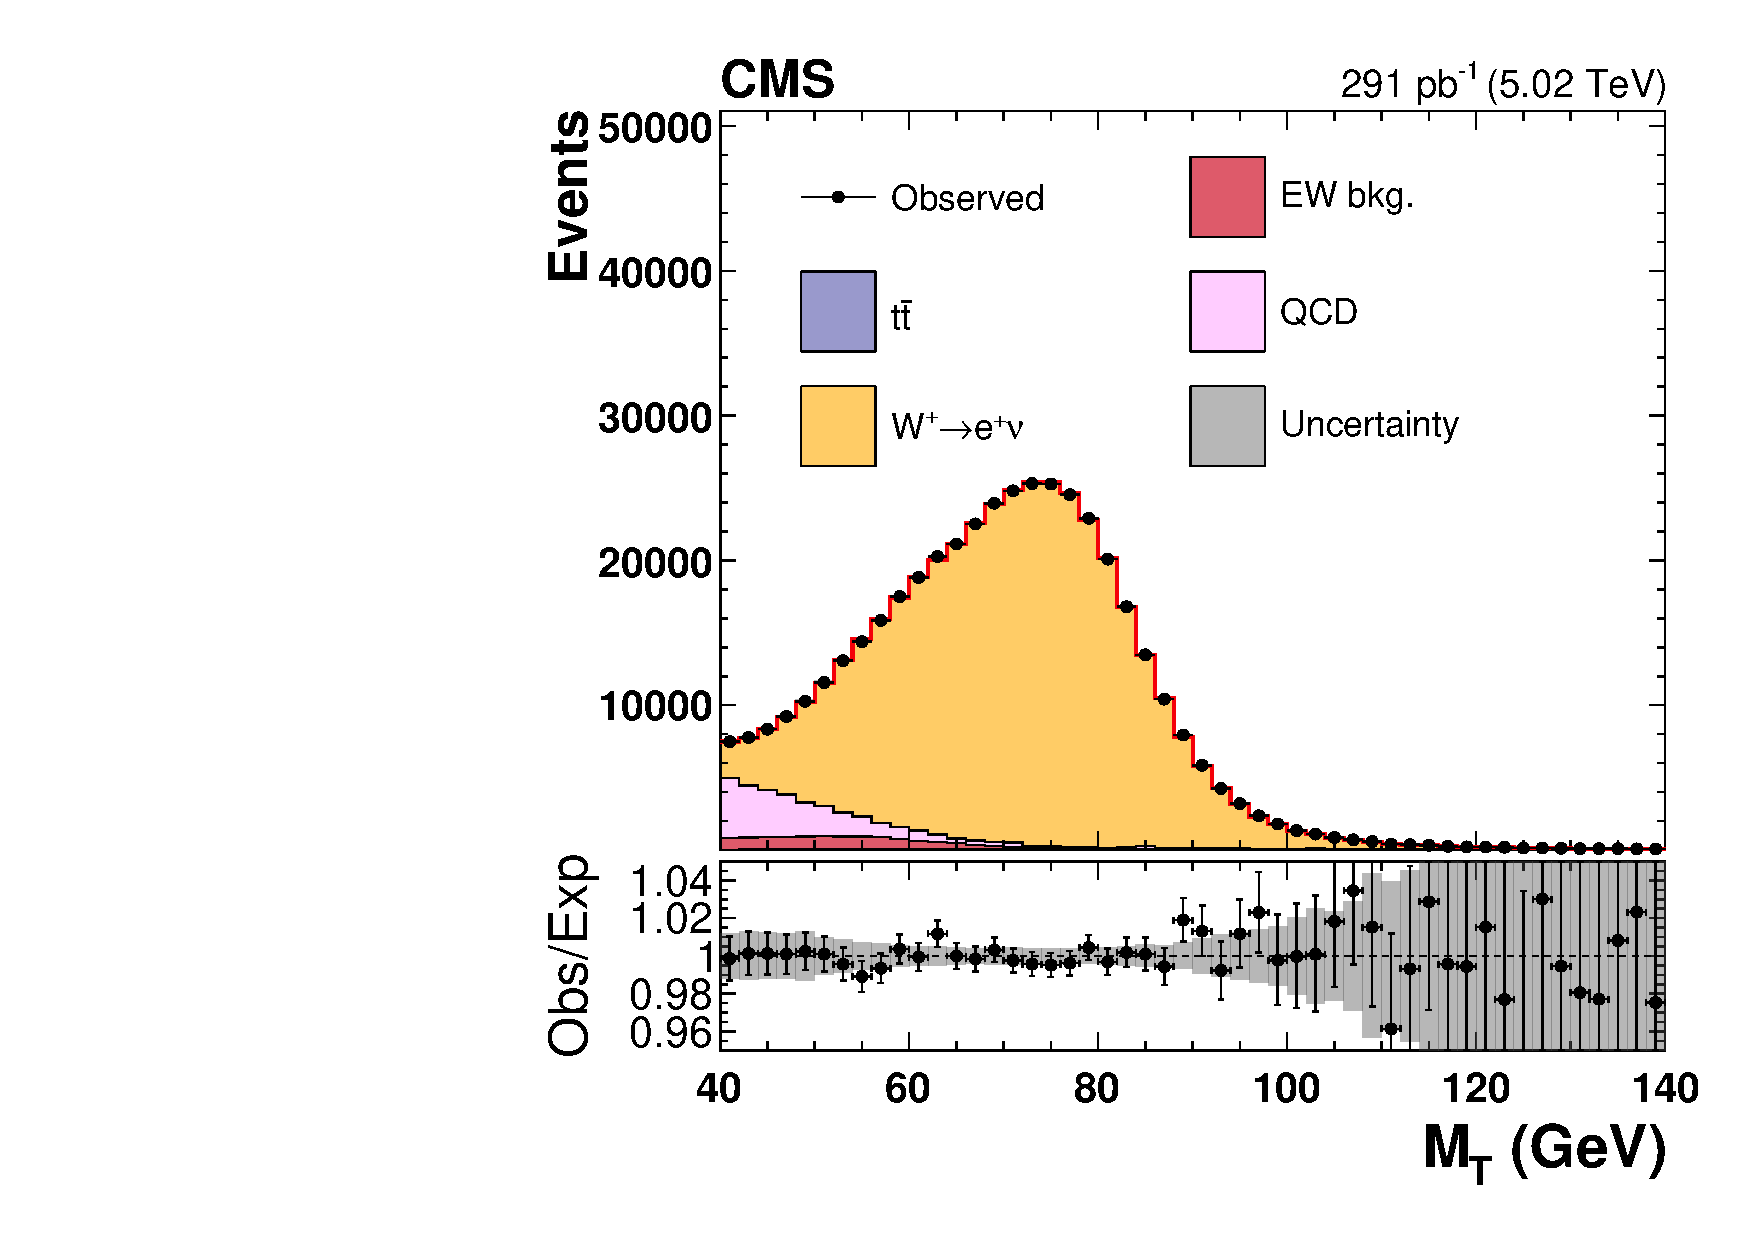
\includegraphics[width=0.49\textwidth]{plots/W/wpefit5.pdf}
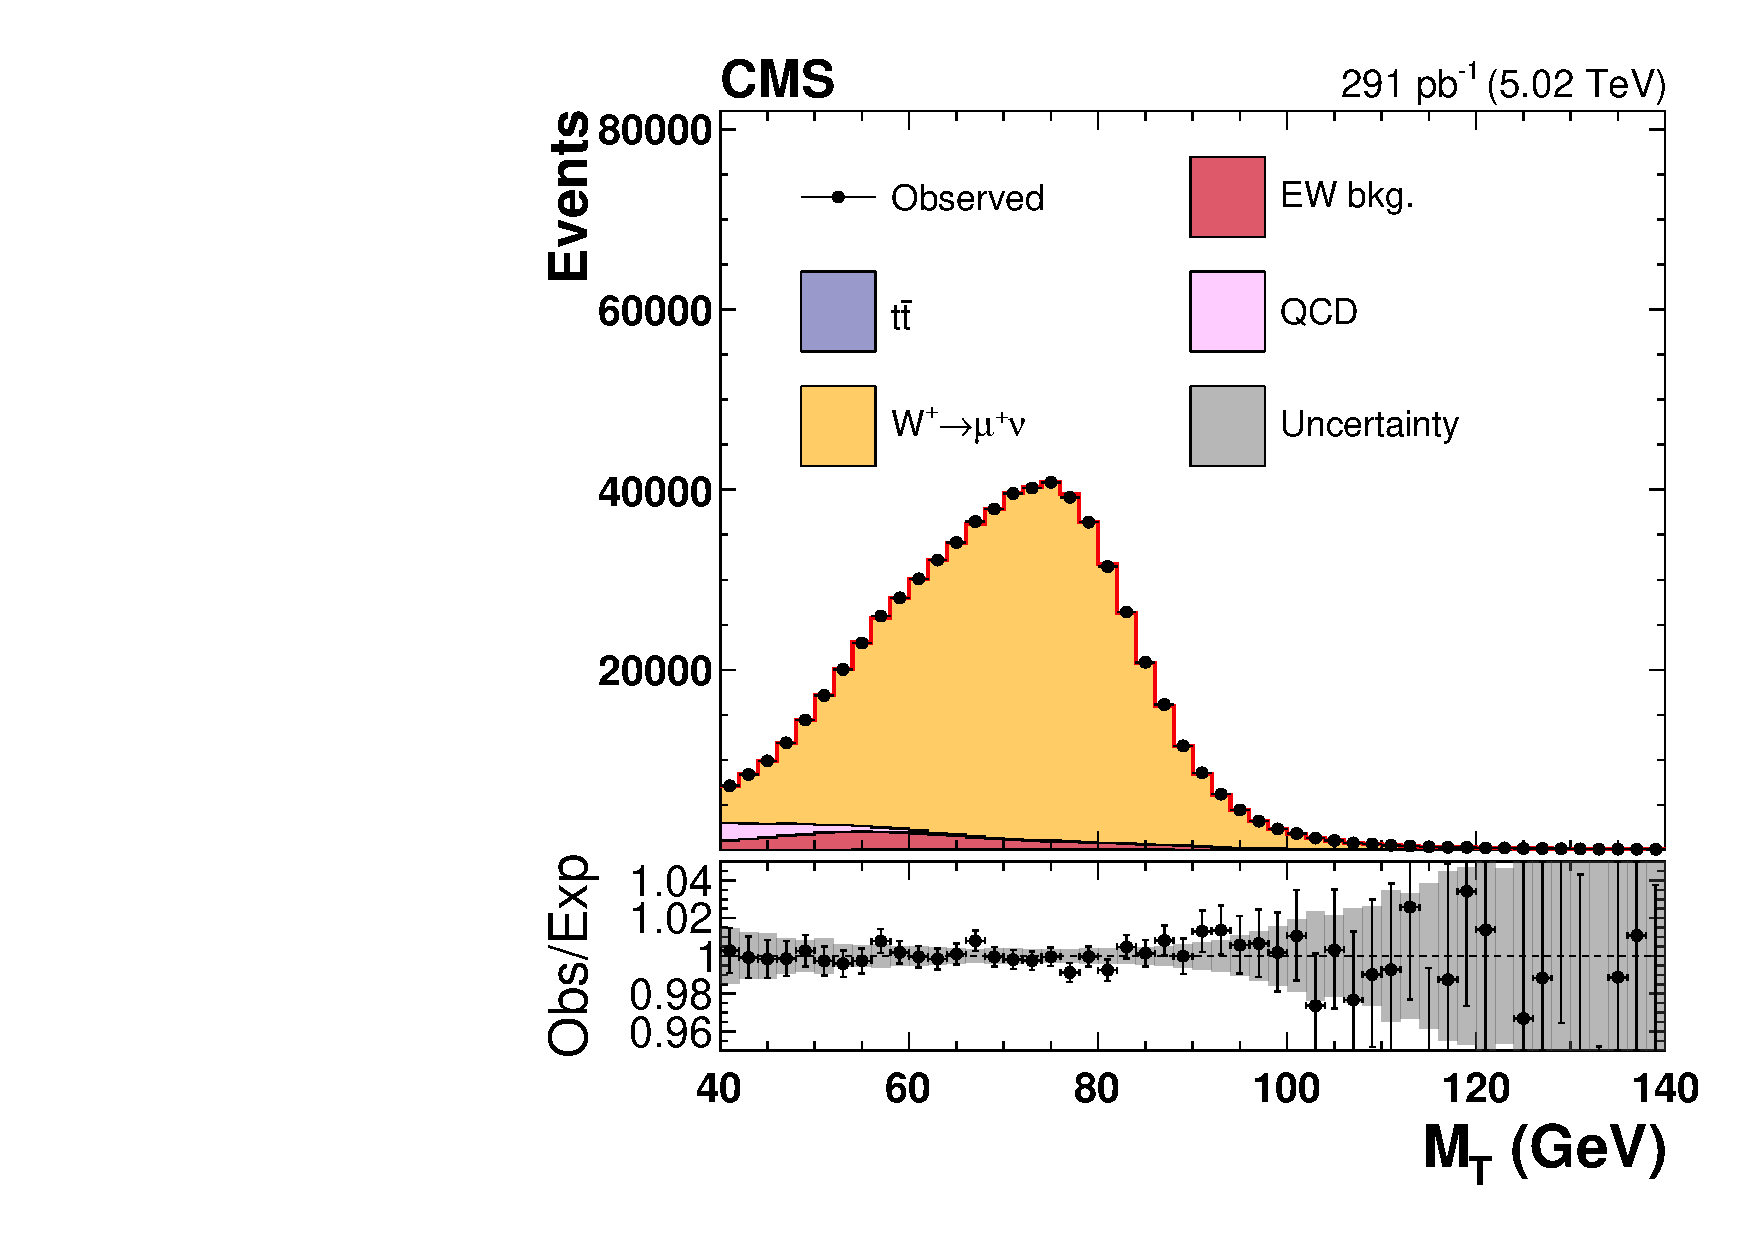
\includegraphics[width=0.49\textwidth]{plots/W/wpmfit5.pdf}
\caption{Distributions of \mt in the $\W^{+}$ signal selection for electron (left) and muon (right) final states for the $pp$ collisions at $\sqrt{s}=13\TeV$ (upper) and $\sqrt{s}=5.02\TeV$ (lower). The histograms for EW backgrounds include the contributions from Drell--Yan, $W \to \tau\nu$, and diboson processes. The predicted yields are shown with their best-fit normalizations from the fit. The bottom panel in each figure shows the ratio of the number of events observed in data to that of the total signal and background predictions.}
\label{fig:signal_wp}
\end{figure*}
\begin{figure*}[htb]
\centering
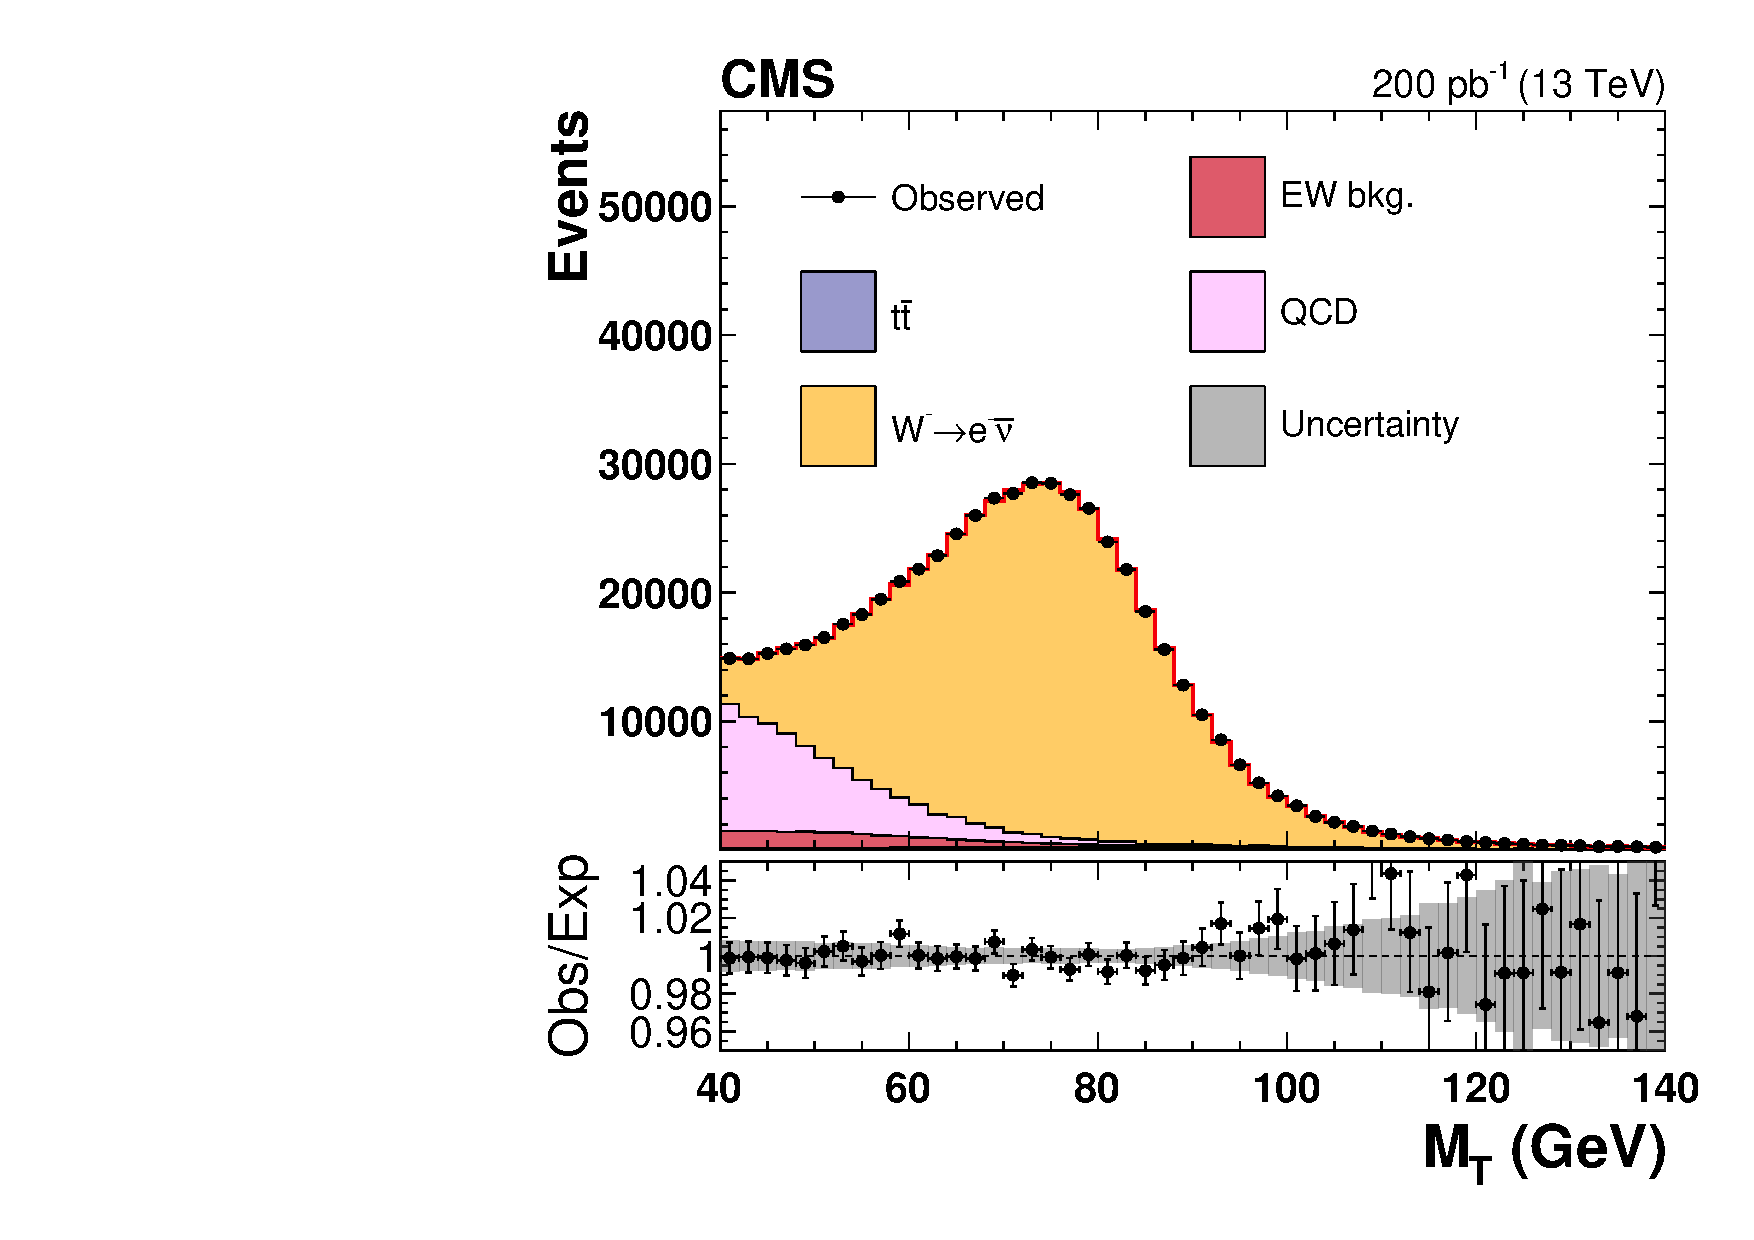
\includegraphics[width=0.49\textwidth]{plots/W/wmefit13.pdf}
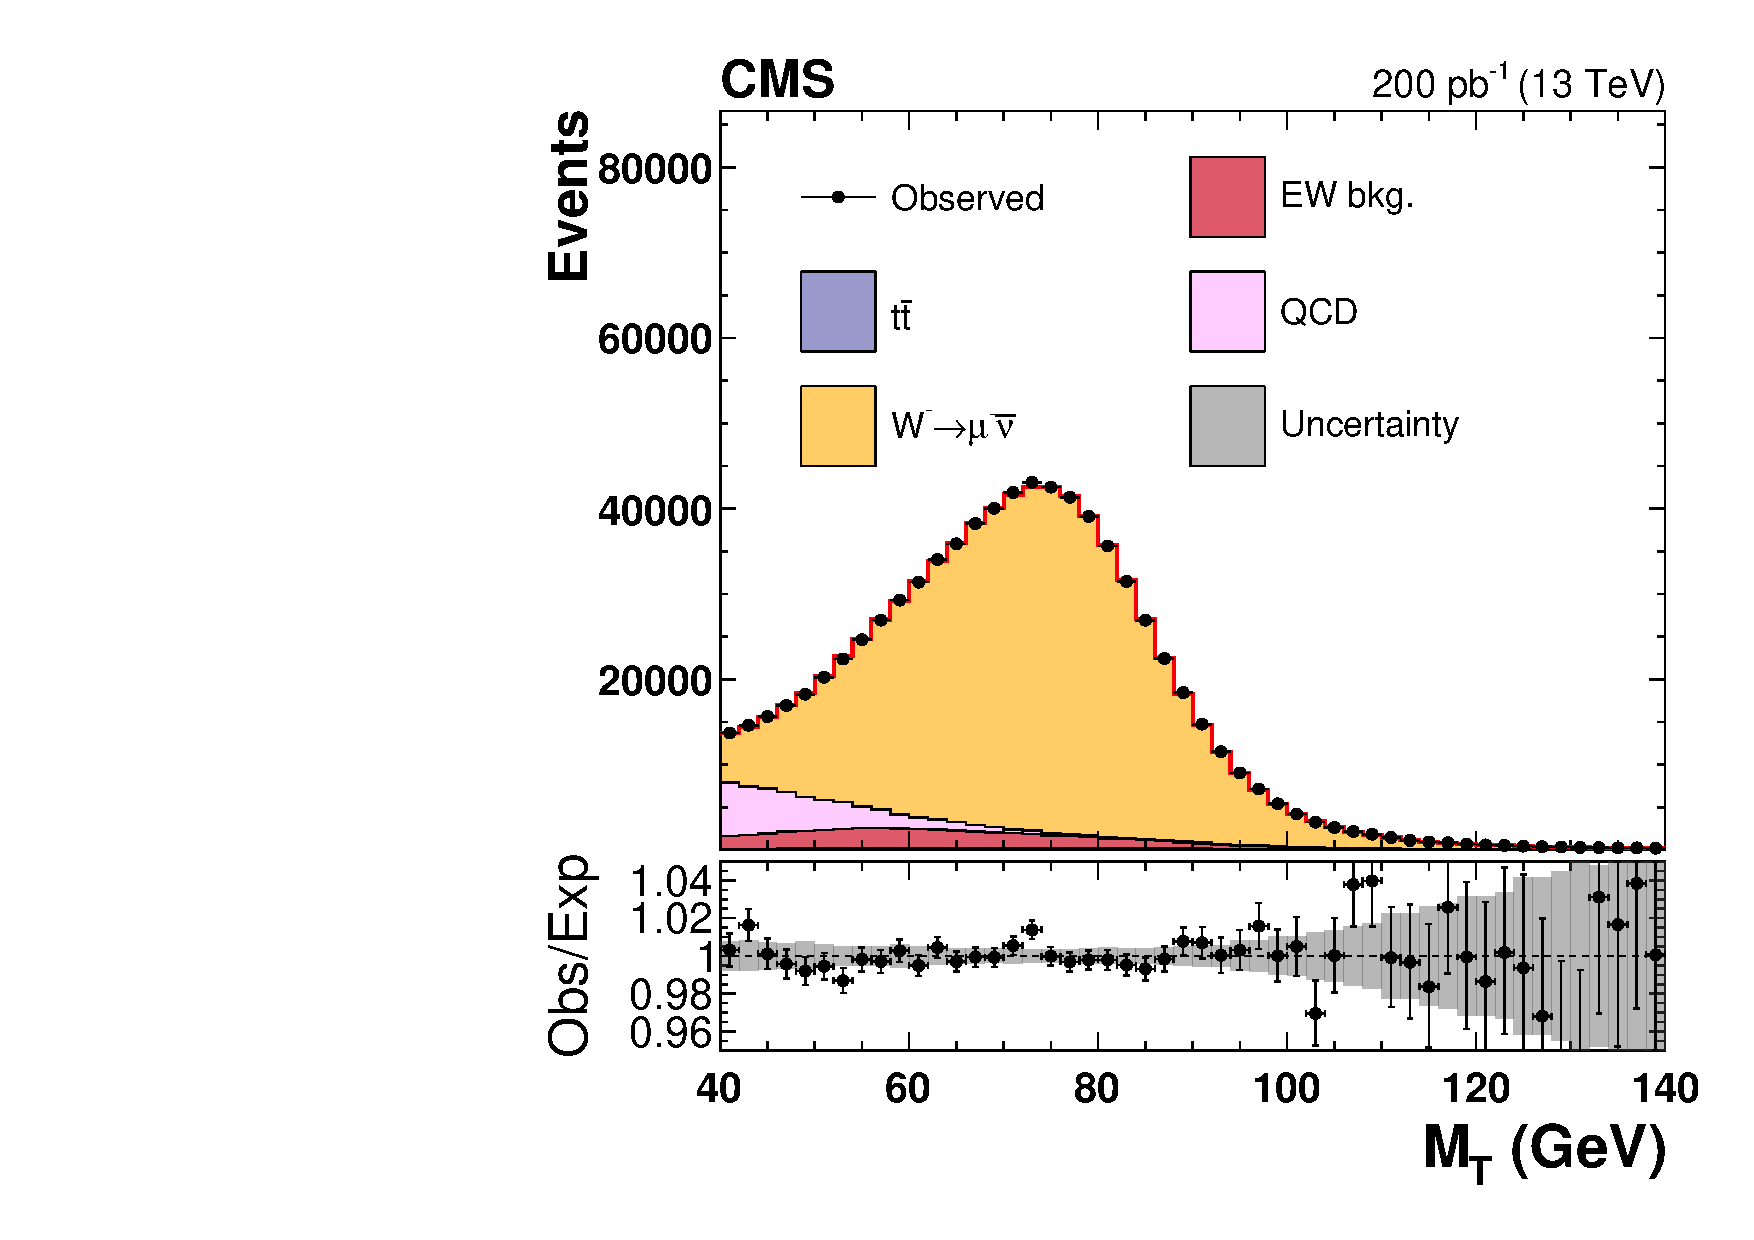
\includegraphics[width=0.49\textwidth]{plots/W/wmmfit13.pdf}
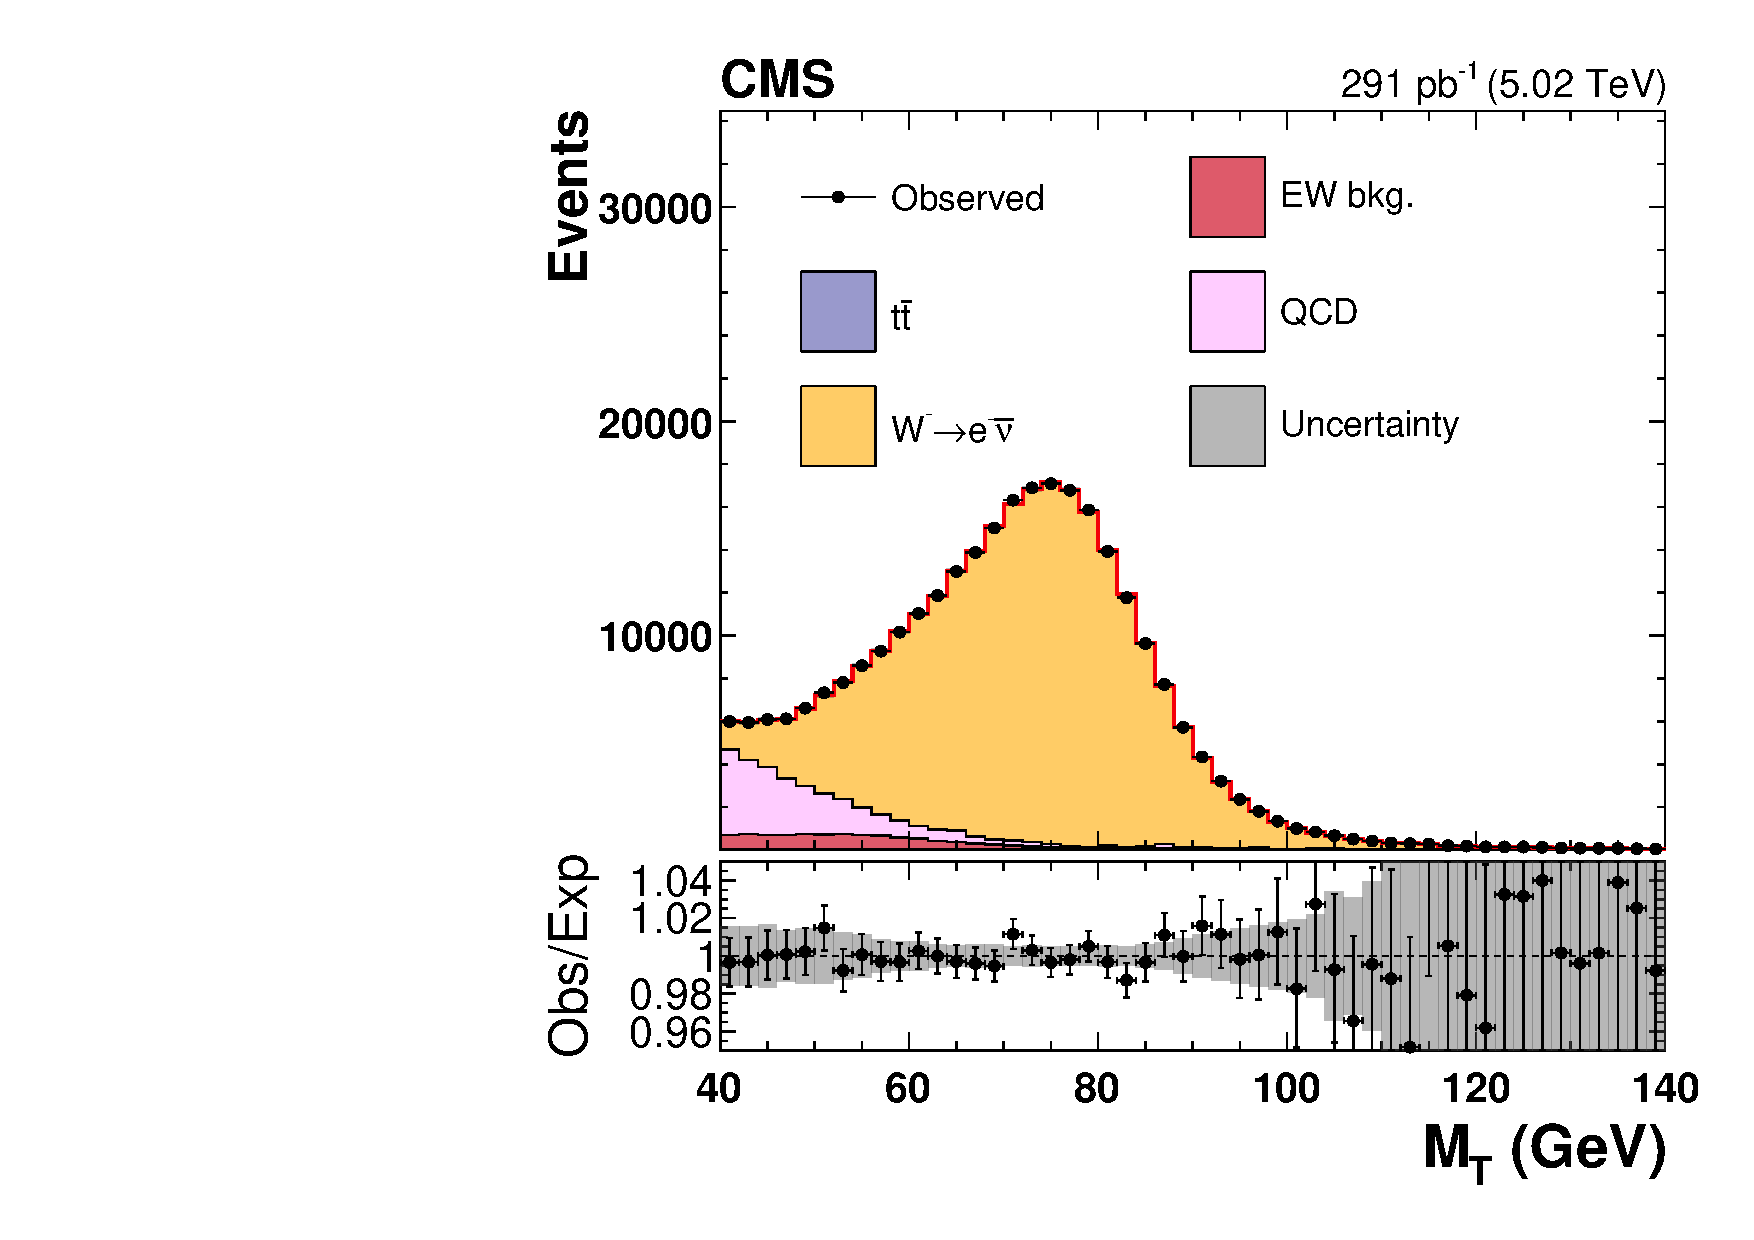
\includegraphics[width=0.49\textwidth]{plots/W/wmefit5.pdf}
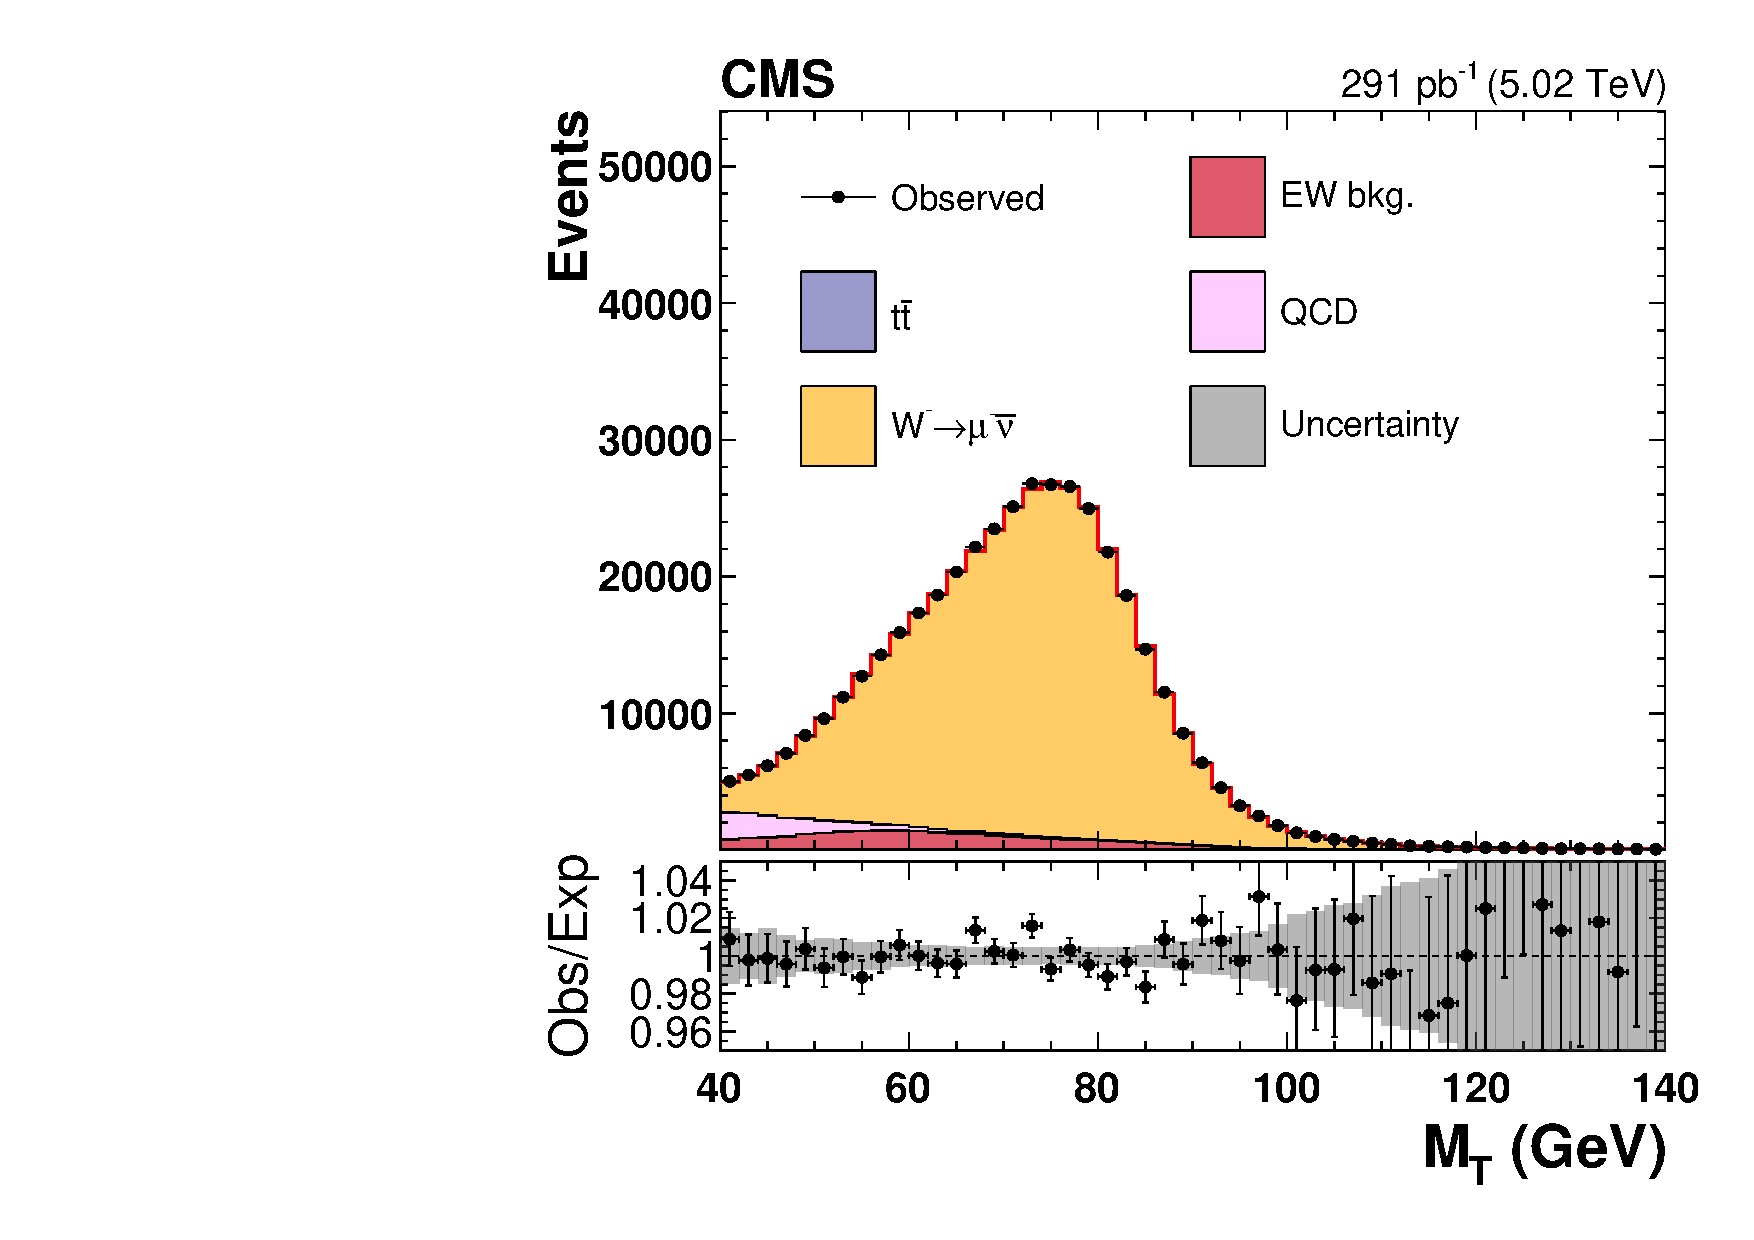
\includegraphics[width=0.49\textwidth]{plots/W/wmmfit5.pdf}
\caption{Distributions of \mt in the $\W^{-}$ signal selection for electron (left) and muon (right) final states for the $pp$ collisions at $\sqrt{s}=13\TeV$ (upper) and $\sqrt{s}=5.02\TeV$ (lower). The histograms for EW backgrounds include the contributions from Drell--Yan, $W \to \tau\nu$, and diboson processes. The predicted yields are shown with their best-fit normalizations from the fit. The bottom panel in each figure shows the ratio of the number of events observed in data to that of the total signal and background predictions.}
\label{fig:signal_wm}
\end{figure*}